%
% LaTe template Masters thesis at IITB
%
% Created by Lakshya Kumar
%
% The official requirement has been persisted with, even if some things could look better some other way.
% Tamper with any of the settings as you see fit and, more importantly, as your guide sees fit.
% Most sections have comments. A lot of stuff is explained in Chapter 1 regarding how to use this template.
% Code snippets for inserting figures, tables and equations are also there in Chapter 1
% Hopefully, this will make report making a little easier.
%

% OK. Here goes.

% Preamble

% Official font size is 12. I thought 11 looked better.
% A4 paper size
% Template for one sided printing of the thesis
\documentclass[12pt, a4paper, oneside]{book}

% Set of packages included. These are all the packages I required, maybe some would be unnecessary and some might be missing. 
% Add any new packages you use over here.
\usepackage{enumitem}
\usepackage{etex}
\usepackage[utf8]{inputenc}
\usepackage{setspace}
\usepackage{amsmath,amsfonts,amssymb,amscd,amsthm,xspace}
\usepackage{titlesec}
\usepackage{vmargin}
\usepackage{fancyhdr}
\usepackage{caption}
\usepackage{subcaption}
\usepackage{multirow}
\usepackage{multicol}
\usepackage{url}
\usepackage{tikz}
\usepackage{tabularx}
\usepackage{graphicx}
\usepackage{epstopdf}
\usepackage{booktabs}
\usepackage{rotating}
\usepackage{listings}
\usepackage{framed}
\usepackage{xcolor}
\usepackage{pgfplots}
\usepackage{verbatim}
\usepackage{amsmath}
\usepackage{adjustbox}
\usepackage[linesnumbered,ruled,vlined]{algorithm2e}
\usepackage{algorithmic}
\usepackage{pdfpages}
 %\usepackage{floatrow}%
% Define bar chart colors
\definecolor{bblue}{HTML}{000000}
\definecolor{ggreen}{HTML}{909497}
\definecolor{rred}{HTML}{ 515A5A }
\definecolor{ppurple}{HTML}{000000}

%\usepackage[centerlast,small,sc]{caption}
\usepackage[square, numbers, comma, sort&compress]{natbib} % Standard reference style with [3], [4] type numbers in the text and entries sorted according to order of appearance in the References
\usepackage[pdfpagemode={UseOutlines},bookmarks=true,bookmarksopen=true,bookmarksopenlevel=0,bookmarksnumbered=true,hypertexnames=false,colorlinks,linkcolor={black},citecolor={black},urlcolor={black},pdfstartview={FitV},unicode,breaklinks=true]{hyperref}
\hypersetup{urlcolor=black, colorlinks=true} % colors hyperlinks in blue - change to black if annoying

% Math operator definition - may not be required
% If any new operators are required, defien them here
\DeclareMathOperator*{\argmin}{argmin}

\title{\thesisTitle}
\author{\authorName}
\date{\today}

% Currently chapter title has been centered, to left align the chapter title and number, change \centering to \flushleft
\titleformat{\chapter}[display]
  {\normalfont\huge\bfseries\centering}
  {\chaptertitlename\ \thechapter}{18pt}{\Huge}

\setmarginsrb   { 3.0cm}  % left margin
                { 1.5cm}  % top margin
                { 2.0cm}  % right margin
                { 2.2cm}  % bottom margin
                { 0.3cm}  % head height
                { 1.2cm}  % head sep
                { 0.3pt}  % foot height
                { 1.0cm}  % foot sep
                
\newcommand{\ie}{i.\,e.~}
\newcommand{\Ie}{I.\,e.~}
\newcommand{\eg}{e.\,g.~}
\newcommand{\Eg}{E.\,g.~}

% End of the Preamble

% Actual document begins
\begin{document}

\newcommand{\HRule}{\rule{\linewidth}{0.5mm}} % New command to make the lines in the title page

% Import all the variable values from Details.tex
% This file contains all the user specific things that need to be changed such as the thesis title, author name etc. 


\newcommand{\thesisTitle}{Constraints on Permission for Making Safe App Execution}

\newcommand{\degree}{\textbf{Master of Technology (M.Tech)} }

\newcommand{\authorName}{\textbf{Dharmendra Kumar}}

\newcommand{\rollNo}{\textbf{163050032}}

\newcommand{\dept}{Department of Computer Science \& Engineering}

\newcommand{\college}{Indian Institute of Technology Bombay}

\newcommand{\currentyear}{2018}

\newcommand{\currentmonth}{June}

\newcommand{\supervisorOne}{\textbf{Prof. R.K. Shyamasundar}}

\newcommand{\supervisorTwo}{Prof. Supervisor Two}

\newcommand{\examinerOne}{\textbf{Prof. Virendra Singh}}

\newcommand{\examinerTwo}{\textbf{Prof. G. Sivakumar}}

\newcommand{\chairman}{Prof. Chairman}

% Use roman page numbering style (i, ii, iii, iv...) for the pre-content pages
\frontmatter

% Line spacing of 1.5 as per IIT requirement. If you think it looks too spaced out, use 1.3
% I think 11 pt font with 1.3 spacing looks quite good
\setstretch{1.5}

% Import all the pages in the front matter
% This file contains the templates for the first few pages of the thesis including 
% 1. Title page
% 2. Dedication
% 3. Dissertation approval
% 4. Declaration of authorship
% 5. Abstract


%   1. TITLE
\newcommand{\titlePage}{

% No page number
\thispagestyle{empty}
\begin{center}
% thesis title
\vspace*{15px}
{\Huge\bfseries \thesisTitle}\\[1.0cm] 

% submitted in partial fulfillment etc.
%\text{M. Tech. Dissertation}

\textit{Submitted in partial fulfillment of the requirements of the degree of\\[0.2cm] \degree}\\[1.0cm]
 
% author
\textit{by}\\[0.2cm]
\authorName \\[0.2cm] \textit{\textbf{Roll no.}} \rollNo \\[2.0cm]

% supervisor
\textit{Supervisor:}\\[0.2cm]
% or
% \textit{under the supervision of}\\[0.2cm]
\supervisorOne \\[2.0cm]

% iit-b logo

\includegraphics[width=0.25\textwidth]{iitb_logo.jpg}

\vspace*{5px}
% department and college
\dept\\
\college\\
% year
\currentyear\\[0.1cm] 
\end{center}
\clearpage
}
%   2. DEDICATION
%\newcommand{\dedication}{
%\thispagestyle{empty}
%\vspace*{75px}
%\begin{center}\large{\textit{Dedicated to ...}}\end{center}

%\clearpage
%}
%   3. DISSERTATION APPROVAL

\newcommand{\approval}{
% if you use a dedication, then use a page number with the plain page style
\thispagestyle{plain}
% else, use no page number with the empty page style
%\thispagestyle{empty}


% page title
\begin{center}{\huge\bf Dissertation Approval\par}\end{center}

\vspace*{15px}

\noindent This project report entitled 
% title
\textbf{``\thesisTitle"}, submitted by 
% author
\authorName ~(Roll No.  \rollNo), is approved for the award of degree of 
% degree
\degree 
~in 
% branch
Computer Science \& Engineering.\\[1.0cm]
% examiners and supervisors
\vspace*{35px}
\begin{center}
\rule{150pt}{2pt}\\
\textbf{Prof. R.K. Shyamasundar}\\
Dept. of CSE, IIT Bombay\\
Supervisor\\[1.5cm]
\end{center}
\vspace*{10px}
\noindent \rule{150pt}{2pt} \hfill \rule{150pt}{2pt}\\
\textbf{Prof. G. Sivakumar} \hfill \textbf{Prof. Bernard Menezes}\\
Dept. of CSE, IIT Bombay \hfill Dept. of CSE, IIT Bombay\\
Internal \& External Examiner \hfill Internal Examiner\\[1.0cm]

\vspace*{30px}
\noindent \textbf{Date:} ...... \currentmonth { } \currentyear\\[0.3cm]
\textbf{Place:}\quad\rule{0.4\textwidth}{.3pt} 

% start a new page
\clearpage
}

%   4. DECLARATION OF AUTHORSHIP
\newcommand{\authorship}{
\thispagestyle{plain}

\begin{center}{\huge\bf Declaration of Authorship\par}\end{center}

\vspace*{15px}

% institute declaration text
\noindent I declare that this written submission represents my ideas in 
my own words and where others' ideas or words have been included, I have adequately cited and 
referenced the original sources.  I also declare that I have adhered to all principles of academic 
honesty and integrity and   have   not   misrepresented   or   fabricated   or   falsified   
any   idea/data/fact/source   in   my submission.  I understand that any violation of the above 
will be cause for disciplinary action by the Institute and can also evoke  penal action from the 
sources which have thus not been properly cited or from whom proper permission has not been taken when needed.

\vspace*{15px}

% signature
\begin{flushright}
{Signature: ......................................\\[0.4cm]}

% author name
{\textbf{\authorName}\\[0.0cm]\rollNo\\[2.0cm]}

\end{flushright}
% date
\begin{flushleft}
{Date: ...... \currentmonth { } \currentyear\\}
\end{flushleft}


% start a new page
\clearpage 
}

%   5. ABSTRACT
\newcommand{\abstractpage}{
\thispagestyle{plain}

% header-type text for the abstract - optional
% \small {\noindent\authorName/ \supervisorOne{ }(Supervisor): \textbf{``\thesisTitle"}, \textit{MTech Project}, \dept, \college, \currentmonth { } \currentyear.}\\[0.0cm]
% \HRule\\[0.2cm]


% \vspace*{10px}

\begin{center}{\huge{\textit {Abstract}}\par}\end{center}

\vspace*{10px}

% Abstract text - Type abstract here
In recent past smart-phones have become very popular due to their utility in obtaining online services and increasing level of user convenience. The cost of smart-phones is falling and increasing number of laymen are using such devices installed with utility applications. Android operating system runs on nearly 82\% of these smart-phones available today. As in the case of desktop operating systems, mobile operating systems too are prone to viruses and malware and there is a steep increase in malicious Apps on Android's application store from where the users install their applications. There exists techniques and methods that are developed to check whether an application is benign or malicious. Applications are checked before they are uploaded to the applications store. The statistics shows that the existing approaches are falling short. Most of the works classify applications into categories based on certain models. Accuracy of these models has direct impact on the security of the user data these applications have access to on a smart-phone. Sometimes malicious applications are also classified as benign. In such cases, there can be serious security breaches as the application makes its way to users' smart-phones via application store. The main idea of our approach is to restrict the malicious behaviour of applications to provide the security to user's private data and device itself. We have done dynamic and static analysis of applications to know the behaviour of applications. We have build classification models using various machine learning techniques to classify the applications as benign or malicious. If applications are classified as malicious, we have restricted its malicious behaviour without modifying apk file. We have used wrappper around the applications such that applications work normally even after restrictions.
\\[0.2cm]

% Index terms
% \noindent \textbf{Index terms}: Sentiment 

% Start a new page
\clearpage 
}

\titlePage

\setcounter{page}{1}
% \dedication

\addcontentsline{toc}{chapter}{Dissertation Approval}

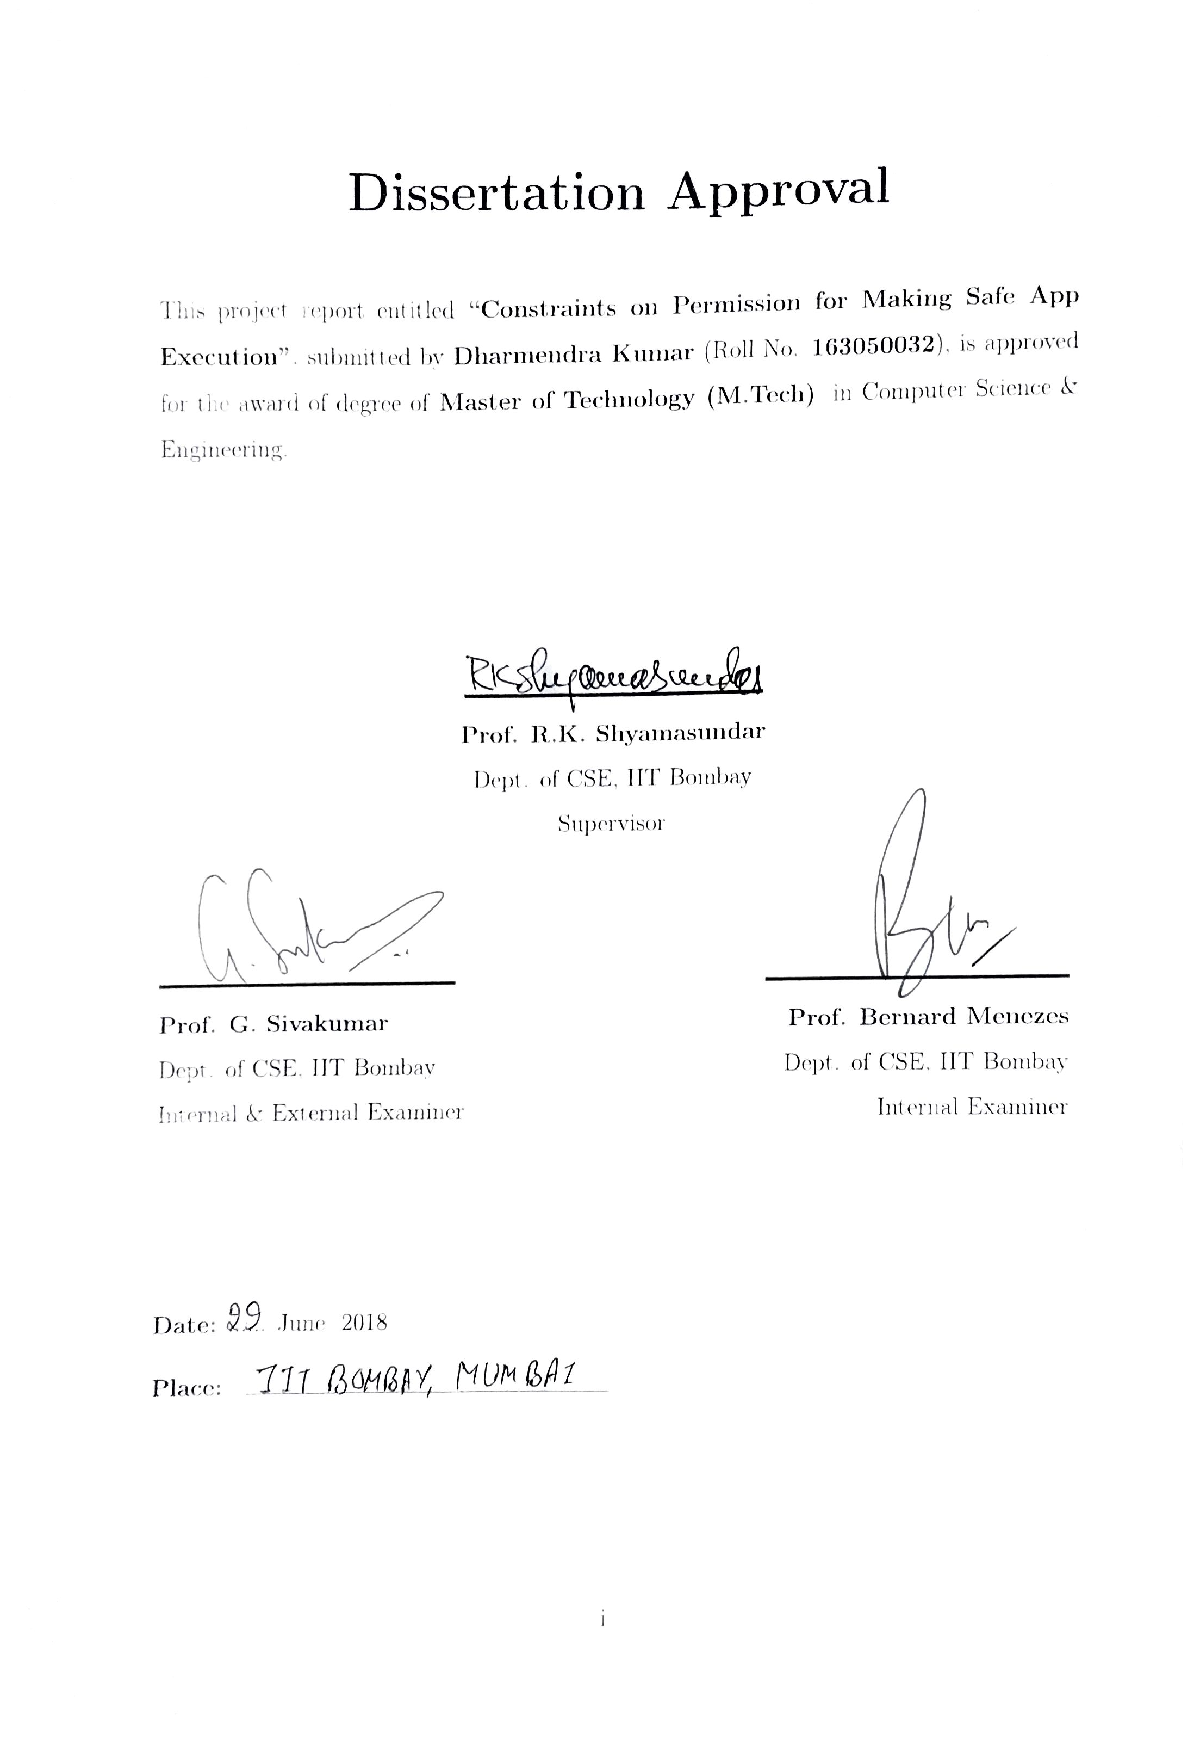
\includepdf[pages=1,trim=0mm 0mm 35mm -20mm]{d_mtp1}
    


\addcontentsline{toc}{chapter}{Declaration of Authorship}

\includepdf[pages=2,trim=0mm 0mm 35mm -20mm]{d_mtp}


\addcontentsline{toc}{chapter}{Abstract}
\abstractpage

\pagestyle{fancy}

% Set the left side page header to "Contents"
\lhead{\emph{Contents}} 

% Write out the Table of Contents
\tableofcontents 

% Set the left side page header to "List of Figures"
\lhead{\emph{List of Figures}} 

% Write out the List of Figures
\listoffigures 
\addcontentsline{toc}{chapter}{List of Figures}

% Set the left side page header to "List of Tables"
% \lhead{\emph{List of Tables}} 

% Write out the List of Tables
% \listoftables
% \addcontentsline{toc}{chapter}{List of Tables}

\fancyhead{}
\rhead{\thepage}


% Use arabic page numbering style (1, 2, 3...) for the body of the report
\mainmatter

% Import the Chapters
% Main chapter title
\chapter{Introduction}
\label{ch:intro}

% This is for the header on each page
\lhead{Chapter 1. \emph{Introduction}}
\thispagestyle{empty}
Android mobile devices is becoming very popular due to ease of use and its user-friendliness User Interface (UI). There is monopoly of Android in mobile device market. Nearly 82\% of smartphones run Android Operating System \cite{smartphoneos} . Due to such a large market share, malware authors are targeting Android mobile devices. The Android is the fastest growing mobile operating system. Unlike Apple's App Store, deploying an application in Google Play Store is much easier. Google takes minimal steps for inspection of applications this allows anyone to publish applications on the Android market. If an application is reported as malware by users, it will then be removed. Due to large market share and easy deployment policy, malware authors are targetting Android. Malware authors are creating malicious application to compromise Android security. According to AO Kaspersky Lab, following Android security issues were in trend in 2016:
\begin{itemize}
    \item Third party applications using super user permissions.
    \item Development of new mechanism to pass security system.
    \item Ransomware i.e encrypting mobile devices.
    \item Continuous improvement in Mobile Banking Trojans.
    \item Deploying malicious application in Google Play Store.
\end{itemize}
\newline
In 2016, Kaspesky Lab detected the following:
\begin{itemize}
    \item 8,534,221 malicious installation packages
    \item 136,786 mobile banking Trojans
    \item 251,114 mobile ransomware Trojans
\end{itemize}

%---------------------------------------------------------------------%

Malicious applications frequently easily passes the security suite of Google's Play Protect security suite, and some applications attracts millions of downloads before Google can find and remove them. Recently the security firm Check Point discovered a new type of Android malware called ``Expensive Wall" hidden in 50 apps in the Play Store. They have been cumulatively downloaded nearly 4.2 million times. Even after Google removed all these applications, Check Point discovered new sample of the malware in the Google Play store. So, we can not only rely on Google Play Protected security suite.\\

Antivirus software is designed to detect, prevent and take action against malicious software. It can either disarm or remove the malicious software. Antivirus scans the file comparing specific pattern in the code against the signature of viruses which already stored in database. If pattern matches, then it is considered as malicious. If a new type of malicious application will come, then it will not be identified by the current antivirus. In that case, from security perspective, application may access user's private data and perform security-sensitive operations on the device.\\

In the current scenario, Android security revolves around the permissions. Applications ask for all the permission that it needs. If required permission is not given to the application, applications does not work properly. Since, applications need all the permission to work we can not restrict particular feature of applications that is causing malicious activity.\\

For providing the security to user's private data and device, our approach is to restrict the behaviour change of Android application and also to restrict them from doing any malicious activity. To achieve our goal we are doing the following things:
\begin{itemize}
    \item We are doing the static and dynamic analysis of the application to gather information about permissions and Application Program Interfaces (APIs). Based on permissions and APIs, we are trying to figure out what can be the possible behaviour of application.
    \item We are building App Classification Model to check whether application is benign or malicious.
    \item We try to restrict the malicious behaviour of application by wrapping the application.
\end{itemize}

%-----------------------------------------------------------------------------------------------------------------%
\paragraph{Organisation:} In the following chapter, that is Chapter 2, we provide background and related work. In Chapter 3, we provide details about the Android software stack architecture and describe only the components of the stack that are relevant to our work. In Chapter 4, we present our approach and also provide analysis of some prominent applications on application store of Android. In Chapter 5, we present our classification models that help us determine/classify whether an app is benign or malicious. In Chapter 6, we show how to restrict malicious intent of an application and also talks about case studies of various applications and  we conclude with possible future work in Chapter 8.
% Main chapter title
\chapter{Background \& Related Work}
\label{ch:sentiment}

% This is for the header on each page
\lhead{Chapter 2. \emph{Related Work \& Background}}
\thispagestyle{empty}
Android operating system has five layer in its software stack. There are multiple applications running on the top of operating system. To provide the security to one application from other applications and to Android operating system from applications Android uses uses virtual machines. Every Android application runs  in its own process, with its own instance of the Dalvik virtual machine (DVM) \cite{wiki:dalvik} / Android Runtime (ART) \cite{androidruntime}. Since, all Android applications run in its own virtural machine, they can not affect the execution of each other and also they can affect Android operating system functionality.

To check the behaviour of Android applications various technique and tools have been developed. Androwarn is a tool to analyze the applications \cite{androwarn}. Androwarn does the static analysis of the application's Dalvik bytecode, represented as Smali and provides the detail about possible malicious behaviour of applications. Flowdroid uses call graphs of the application to analyze the behaviour of the application \cite{arzt2014flowdroid}. Static analysis of application can be done on the basis of permissions it requires \cite{johnson2012analysis}. Another way of static anaysis is to check the behaviour of kernel to provide the behaviour of applications \cite{isohara2011kernel}. 

Droidmate \cite{jamrozik2016droidmate} does the dynamic analysis of application by clicking on various UI element and traces the API calls made. Crowdroid \cite{burguera2011crowdroid} detects the malicious behaviour by analyzing data collected from two sets: one from those from artificial malware created for test purposes, and those from real malware found in the wild. To detect malware in Android applications various methods and techniques have developed. Some of those approaches are:
\\
\\
\textbf{Permission based approach}\\
To stop malware installation permission based system has been developed. While installation applications ask for permission to access sensitive resources. Based on requested permission a classifier has been developed to identify benign and malicious application.
\textbf{Two-layered permission based approach}\\
In this method, they analyzed data from two types of permissions namely \textit{requested permissions} and \textit{used permissions}. After analyzing requested permissions, they make classifier to classify applications int benign and malware. After this classification, they make another classifier by analyzing used permissions to identify malware.\\
\textbf{Malware detection using static feature-based analysis}\\
This approach uses various static information such as permissions, deployment of components, intent message passing and API calls for characterizing the Android application behaviour. After extracting the above information one can
\begin{enumerate}
    \item applies K-means algorithm to classify applications into benign and malware.
    \item can generate a model using KNN classifier for detecting malware.
\end{enumerate}
\textbf{Malware detection using hybrid of static and dynamic analysis}\\
By static analysis, it extracts expected activity switch paths by analyzing both Activity and Function Call Graphs. Then it uses dynamic analysis to traverse each UI elements and explore the UI interactions paths towards sensitive APIs. Using these data, they create a model to detect malware.\\
\textbf{Behaviour-based malware detection system}\\
They firstly gather test data and actual processed data, it processes the data and try to figure out some patterns in the data that can be used to differentiate benign applications and malicious applications. They use different machine learning techniques to find the pattern in the data. After finding the pattern, they make classifier to identify the malware.\\
\textbf{By analyzing usage of sensitive data}\\
In this method, they firstly analyze the flow of sensitive data in benign applications and then try same for malicious applications. From these data, they implements different type of classifier to detect malicious applications.

%-----------------------------------------------------------------------------%

% Main chapter title
\chapter{Android: Architecture, Permissions, APIs}
\label{ch:related}

% This is for the header on each page
\lhead{Chapter 3. \emph{Android: Architecture, Permissions, APIs}}
\thispagestyle{empty}
Android is widely used operating system for moblie devices. In section 3.1, we will discuss about the architecture of android. In section 3.2, we will discuss permissions required by any application to access the sensitive resources. In Section 3.3, we will give brief idea about APIs.
\section{Architecture}
Android is opensource. Android operating system is based on Linux based-software stack \cite{androidplatformarch}. There are mainly five components in Android software stack. These are:
\begin{enumerate}
    \item Linux Kernel
    \item Native Libraries
    \item Android Runtime
    \item Application Framework
    \item Applications
\end{enumerate}
\begin{figure}[!h]
  \centering
  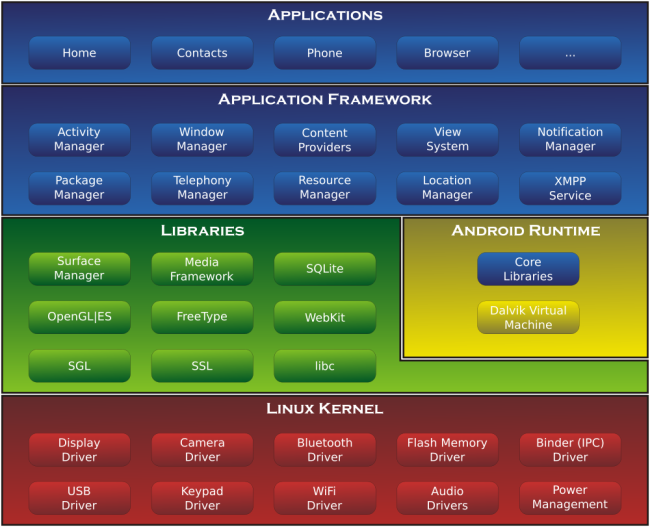
\includegraphics [scale=0.8] {and_arch.png}
  \caption{The Android Software Stack}
  \label{fig:arch}
\end{figure}
\subsection{Linux Kernel}
Linux kernel is root/foundation of the Android platform. Linux kernel is responsible for device drivers, power management, memory management, device management and resource access. Linux kernel includes display driver, camera driver, bluetooth driver, Flash memory driver, Binder (IPC) driver, USB driver, kepad driver, WiFi driver and Audio Driver.

\subsection{Native Libraries}
Native libraries sits on the top of Linux kernel. Some of native libraries are WebKit, OpenGL, FreeType, SQLite, Media, C runtime library (libc), etc. The WebKit is used for browser support, SQLite is used for database, FreeType is used for font support, Media is used for playing and recording audio and video formats.

\subsection{Android Runtime}
Android Runtime contains some core libraries and DVM (Dalvik Virtual Machine) which is responsible to run android application. DVM is similar to JVM but it is more optimized for mobile devices. It comsumes less memory and provides fast performance. ART is written to run multiple virtual machines on low-memory devices. Some of the major features of ART includes the following:
\begin{itemize}
    \item Ahead-of-time (AOT) and just-in-time (JIT) Compilation.
    \item Optimized garbage collection (GC).
    \item Better debugging support, including a dedicated sampling profiler, detailed diagnostic exceptions and crash reporting, and the ability to set watchpoints to monitor specific fields.
\end{itemize}

\subsection{Android Framework}
Android Framework sits on the top of Native libraries and Android runtime. Android framework contains Content provider, View system, Activity manager, Window manager, Telephony manager, resource manager, location manager and XMPP service.

\subsection{Applications}
Last layer of the Android Platform Architecture is applications. It contains applications. All applications such as home, contact, settings, email, dialer, calendar, camera, etc. are using Android framework that uses Native libraries and Android runtime. Android runtime and native libraries are using linear kernel.


%---------------------------------------------------------------------%
%---------------------------------------------------------------------%
\section{Permissions}
If an Android application wants to use any resources such as camera, internet, location, etc., they need permission from the Android operating system to use them. Android marshmallow operating system has more than 200 permissions \cite{androidpermissions}. The main purpose of permission is to protect the user data. Android apps must request permission to access sensitive user data as well as the system features. Depending on the feature, the system might grant the permission automatically or might prompt the user to approve the request. Permissions are divided into several protection level. There are three protection levels that affect third-party apps:
\begin{enumerate}
    \item Normal permissions
    \item Signature permissions
    \item Dangerous permissions
\end{enumerate}
\subsection{Normal Permissions}
Normal permissions are used where an needs to access data or resources outside the app's sandbox but where there is very little risk to the user's privacy or the operation of other apps. According to Android 8.1, following are the list of normal permissions:
\begin{itemize}
    \begin{spacing}{0.9}
    \item \texttt{ACCESS\_LOCATION\_EXTRA\_COMMANDS}
    \item \texttt{ACCESS\_NETWORK\_STATE}
    \item \texttt{ACCESS\_NOTIFICATION\_POLICY}
    \item \texttt{ACCESS\_WIFI\_STATE}
    \item \texttt{BLUETOOTH}
    \item \texttt{BLUETOOTH\_ADMIN}
    \item \texttt{BROADCAST\_STICKY}
    \item \texttt{CHANGE\_NETWORK\_STATE}
    \item \texttt{CHANGE\_WIFI\_MULTICAST\_STATE}
    \item \texttt{CHANGE\_WIFI\_STATE}
    \item \texttt{DISABLE\_KEYGUARD}
    \item \texttt{EXPAND\_STATUS\_BAR}
    \item \texttt{GET\_PACKAGE\_SIZE}
    \item \texttt{INSTALL\_SHORTCUT}
    \item \texttt{INTERNET}
    \item \texttt{KILL\_BACKGROUND\_PROCESSES}
    \item \texttt{MANAGE\_OWN\_CALLS}
    \item \texttt{MODIFY\_AUDIO\_SETTINGS}
    \item \texttt{NFC}
    \item \texttt{READ\_SYNC\_SETTINGS}
    \item \texttt{READ\_SYNC\_STATS}
    \item \texttt{RECEIVE\_BOOT\_COMPLETED}
    \item \texttt{REORDER\_TASKS}
    \item \texttt{REQUEST\_COMPANION\_RUN\_IN\_BACKGROUND}
    \item \texttt{REQUEST\_COMPANION\_USE\_DATA\_IN\_BACKGROUND}
    \item \texttt{REQUEST\_DELETE\_PACKAGES}
    \item \texttt{REQUEST\_IGNORE\_BATTERY\_OPTIMIZATIONS}
    \item \texttt{SET\_ALARM}
    \item \texttt{SET\_WALLPAPER}
    \item \texttt{SET\_WALLPAPER\_HINTS}
    \item \texttt{TRANSMIT\_IR}
    \item \texttt{USE\_FINGERPRINT}
    \item \texttt{VIBRATE}
    \item \texttt{WAKE\_LOCK}
    \item \texttt{WRITE\_SYNC\_SETTINGS}
    \end{spacing}
\end{itemize}
\subsection{Signature Permissions}
The system grants these app permissions at install time, but only when the app that attempts to use a permission is signed by the same certificate as the app that defines the permission. According to Android 8.1, following are the list of signature permissions:
\begin{itemize}
    \begin{spacing}{0.9}
    \item \texttt{BIND\_ACCESSIBILITY\_SERVICE}
    \item \texttt{BIND\_AUTOFILL\_SERVICE}
    \item \texttt{BIND\_CARRIER\_SERVICES}
    \item \texttt{BIND\_CHOOSER\_TARGET\_SERVICE}
    \item \texttt{BIND\_CONDITION\_PROVIDER\_SERVICE}
    \item \texttt{BIND\_DEVICE\_ADMIN}
    \item \texttt{BIND\_DREAM\_SERVICE}
    \item \texttt{BIND\_INCALL\_SERVICE}
    \item \texttt{BIND\_INPUT\_METHOD}
    \item \texttt{BIND\_MIDI\_DEVICE\_SERVICE}
    \item \texttt{BIND\_NFC\_SERVICE}
    \item \texttt{BIND\_NOTIFICATION\_LISTENER\_SERVICE}
    \item \texttt{BIND\_PRINT\_SERVICE}
    \item \texttt{BIND\_SCREENING\_SERVICE}
    \item \texttt{BIND\_TELECOM\_CONNECTION\_SERVICE}
    \item \texttt{BIND\_TEXT\_SERVICE}
    \item \texttt{BIND\_TV\_INPUT}
    \item \texttt{BIND\_VISUAL\_VOICEMAIL\_SERVICE}
    \item \texttt{BIND\_VOICE\_INTERACTION}
    \item \texttt{BIND\_VPN\_SERVICE}
    \item \texttt{BIND\_VR\_LISTENER\_SERVICE}
    \item \texttt{BIND\_WALLPAPER}
    \item \texttt{CLEAR\_APP\_CACHE}
    \item \texttt{MANAGE\_DOCUMENTS}
    \item \texttt{READ\_VOICEMAIL}
    \item \texttt{REQUEST\_INSTALL\_PACKAGES}
    \item \texttt{SYSTEM\_ALERT\_WINDOW}
    \item \texttt{WRITE\_SETTINGS}
    \item \texttt{WRITE\_VOICEMAIL}
    \end{spacing}
\end{itemize}
\subsection{Dangerous Permissions}
Dangerous permissions cover areas where the app wants data or resources that involve the user's private information, or could potentially affect the user's stored data or the operation of other apps. If an app declares that it needs a dangerous permission, the user has to explicitly grant the permission to the app. Until the user approves the permission, your app cannot provide functionality that depends on that permission. According to Android 8.1, following are the list of dangerous permissions:
\begin{itemize}
    \begin{spacing}{0.9}
    \item \texttt{READ\_CALENDAR}
    \item \texttt{WRITE\_CALENDAR}
    \item \texttt{CAMERA}
    \item \texttt{READ\_CONTACTS}
    \item \texttt{WRITE\_CONTACTS}
    \item \texttt{GET\_ACCOUNTS}
    \item \texttt{ACCESS\_FINE\_LOCATION}
    \item \texttt{ACCESS\_COARSE\_LOCATION}
    \item \texttt{RECORD\_AUDIO}
    \item \texttt{READ\_PHONE\_STATE}
    \item \texttt{READ\_PHONE\_NUMBERS}
    \item \texttt{CALL\_PHONE}
    \item \texttt{ANSWER\_PHONE\_CALLS}
    \item \texttt{READ\_CALL\_LOG}
    \item \texttt{WRITE\_CALL\_LOG}
    \item \texttt{ADD\_VOICEMAIL}
    \item \texttt{USE\_SIP}
    \item \texttt{PROCESS\_OUTGOING\_CALLS}
    \item \texttt{BODY\_SENSORS}
    \item \texttt{SEND\_SMS}
    \item \texttt{RECEIVE\_SMS}
    \item \texttt{READ\_SMS}
    \item \texttt{RECEIVE\_WAP\_PUSH}
    \item \texttt{RECEIVE\_MMS}
    \item \texttt{READ\_EXTERNAL\_STORAGE}
    \item \texttt{WRITE\_EXTERNAL\_STORAGE}
    \end{spacing}
\end{itemize}
\section{Application Program Interfaces (APIs)}
The Android API refers to the collection of various software modules which make up the complete Android SDK. If we have to use any functionality of android, then we have to use API corresponding to that functionality.

%\input{Chapters/Chapter03_02}
% Main chapter title
\chapter{Method of App Analysis}
\label{ch:dl}

% This is for the header on each page
\lhead{Chapter 4. \emph{Method of App Analysis}}
\thispagestyle{empty}
In Google Play Store, there are lots of malicious applications. So, we have tried to find the behaviour of application and restrict its malicious intent if any. In section 4.1, we have discussed our approach. In section 4.2, we have discussed about analysis of some applications.
\section{Design Approach}
There are nearly 3.6 million applications on Google play store \cite{availableapp}. Not all the applications are benign on the Google play store. Some applications may have security issues. Android also supports installation of application from third and third party application can not be trusted. So, we have proposed a mechanism to determine the behaviour of application. If we find behaviour of application as malicious, then we have to restrict the malicious behaviour of applications. We are doing the whole process in following three phases:
\begin{enumerate}
    \item Analysis of application.
    \item Determining behaviour of application.
    \item Restricting malicious intent of application.
\end{enumerate}
\begin{figure}[!h]
  \centering
  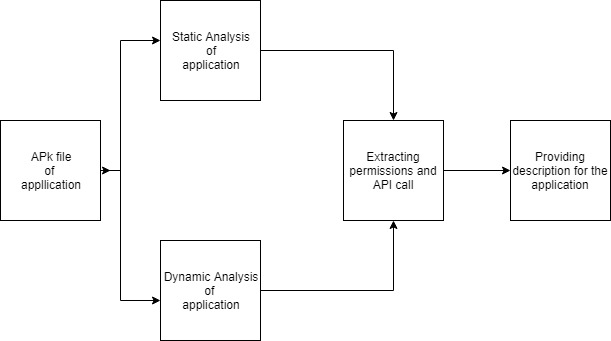
\includegraphics [scale=0.6] {archwork1.jpg}
  \caption{Workflow of analysis phase}
  \label{fig:archwork1}
\end{figure}

We are doing static and dynamic analysis of applications. For analyzing the application we are using Droidmate \cite{jamrozik2016droidmate}, RiskIndroid \cite{merlo2017riskindroid} and AndroPyTool \cite{andropytoool}. From the analysis we are extracting the permissions and API calls from the applications. After seeing the permissions required by applications and API calls it is invoking, we are proposing the description of the application. Workflow for analysis phase is shown in Figure \ref{fig:archwork1}.

\\
Using the analyzed data of applications whose class is known ( it is known that whether application is benign or malicious), we are developing the classification model with the help of various machine learning techniques such as Logistic Regression, Support Vector Machine, Neural Network and Random Forest. Once the model is built, we are using that classification model to determine the class of applications that we have analyzed. Workflow for classification phase is shown in Figure \ref{fig:archwork2}
\begin{figure}[!h]
  \centering
  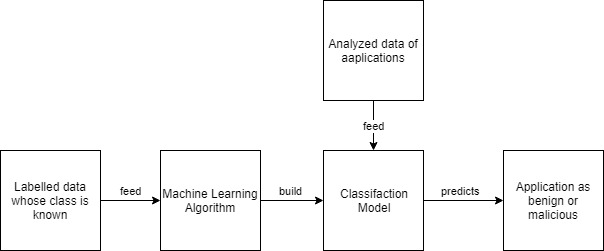
\includegraphics [scale=0.6] {archwork2.jpg}
  \caption{Workflow of classification phase}
  \label{fig:archwork2}
\end{figure}

Once we know that whether applications are malicious or benign, then we only focus of malicious applications. We try to restrict the malicious behaviour or intent of the applications by using a wrapper around the applications. Figure \ref{fig:archwork3} shows the workflow of restriction phase.

\begin{figure}[!h]
  \centering
  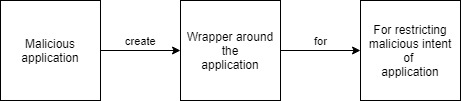
\includegraphics [scale=0.6] {archwork3.jpg}
  \caption{Workflow of restirction phase}
  \label{fig:archwork3}
\end{figure}




%---------------------------------------------------------------------%
\section{Analysis of Application}
In dynamic analysis, we are extracting several information like Unique APIs found, actionable views seen, unique API+event pairs found, and actionable unique views clicked. We trace the API calls that have been invoked while triggering UI elements. In static analysis, we are extracting information about permissions declared and used in application.

For dynamic analysis, we have used DROIDMATE which is fully automatic test generator for Android application and for static analysis we have used RiskInDroid which is python tool used for reverse engineering, malware and goodware analysis of Android application. We have also used AndoPyTool for both Dynamic and static analysis of applications.
\subsection{Budget Planner}
Budget Planner is an Android application which is used for managing your savings and expenses. Figure \ref{fig:bp} shows the screenshot taken during static analysis and Figure \ref{fig:bp1}  shows the screenshot taken during dynamic analysis of application.
\begin{figure}[!h]
  \centering
  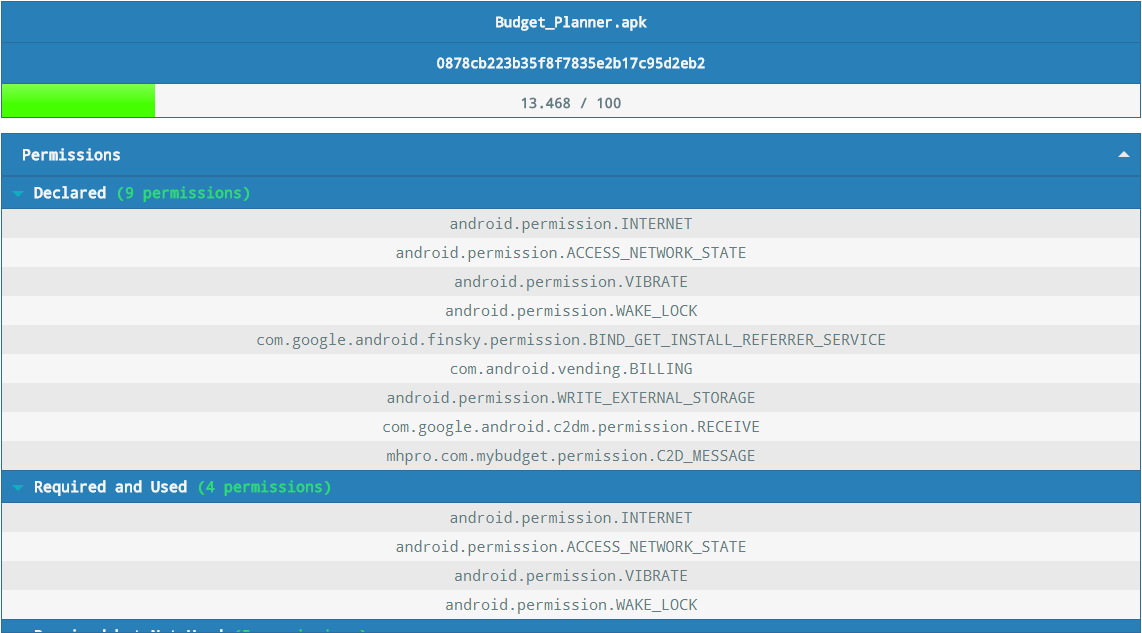
\includegraphics [scale=0.5] {bp.png}
  \caption{Screenshot captured during static analysis of Budget Planner app}
  \label{fig:bp}
\end{figure}
\subsubsection{Permissions}
We have extracted the following 9 permissions during the static analysis of Budget Planner app:\\
\textbf{Required and used} (4 permissions)
\begin{itemize}
    \begin{spacing}{0.9}
    \item \texttt{android.permission.INTERNET} \hfill - Dangerous
    \item \texttt{android.permission.ACCESS\_NETWORK\_STATE} \hfill - Dangerous
    \item \texttt{android.permission.VIBRATE}
    \item \texttt{android.permission.WAKE\_LOCK}
    \end{spacing}
\end{itemize}
\textbf{Required but not used} (5 permissions)
\begin{itemize}
    \begin{spacing}{0.9}
    \item \texttt{com.google.android.finsky.permission.BIND\_GET\_INSTALL\_REFERRER\_SERVICE}
    \item \texttt{com.android.vending.BILLING}
    \item \texttt{android.permission.WRITE\_EXTERNAL\_STORAGE} \hfill - Dangerous
    \item \texttt{com.google.android.c2dm.permission.RECEIVE}
    \item \texttt{mhpro.com.mybudget.permission.C2D\_MESSAGE}
    \end{spacing}
\end{itemize}
\begin{figure}[h]
	\centering
	\begin{subfigure}[h]{0.45\textwidth}
		\centering
		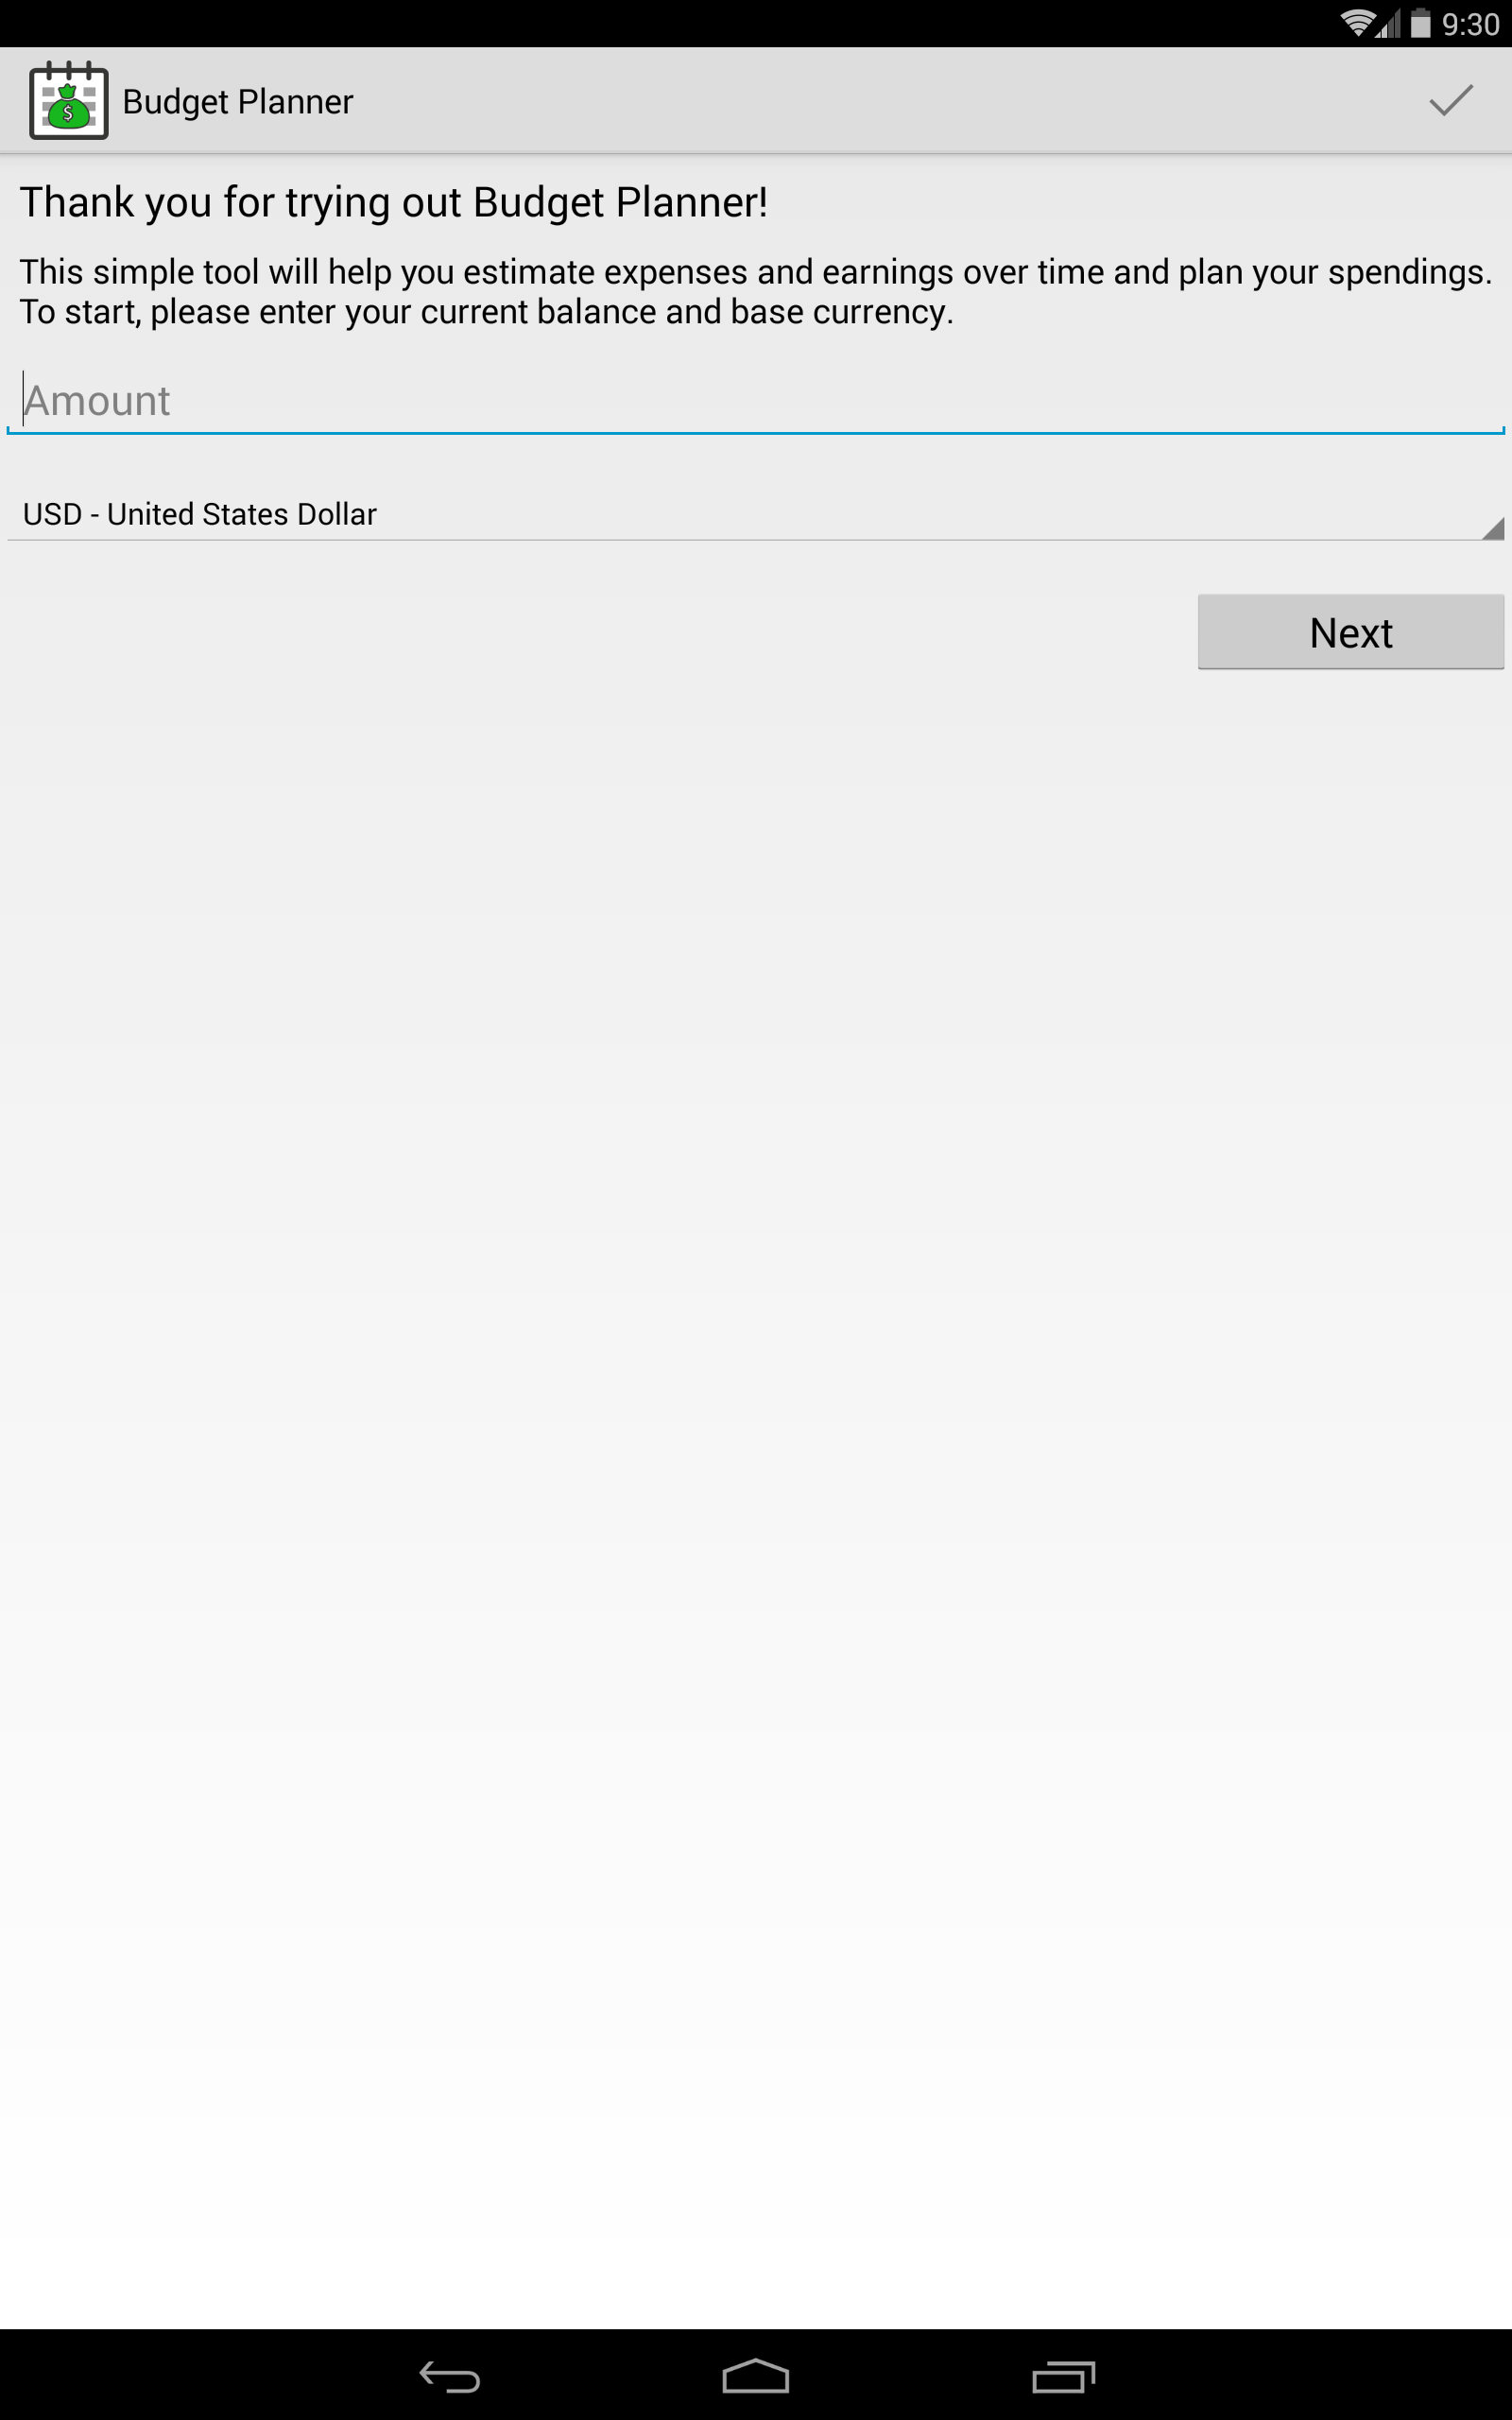
\includegraphics[width=\textwidth]{bp1.png}
		\caption{Budget Planner screenshot-1}
	\end{subfigure}
	\hfill
	\begin{subfigure}[h]{0.45\textwidth}
		\centering
		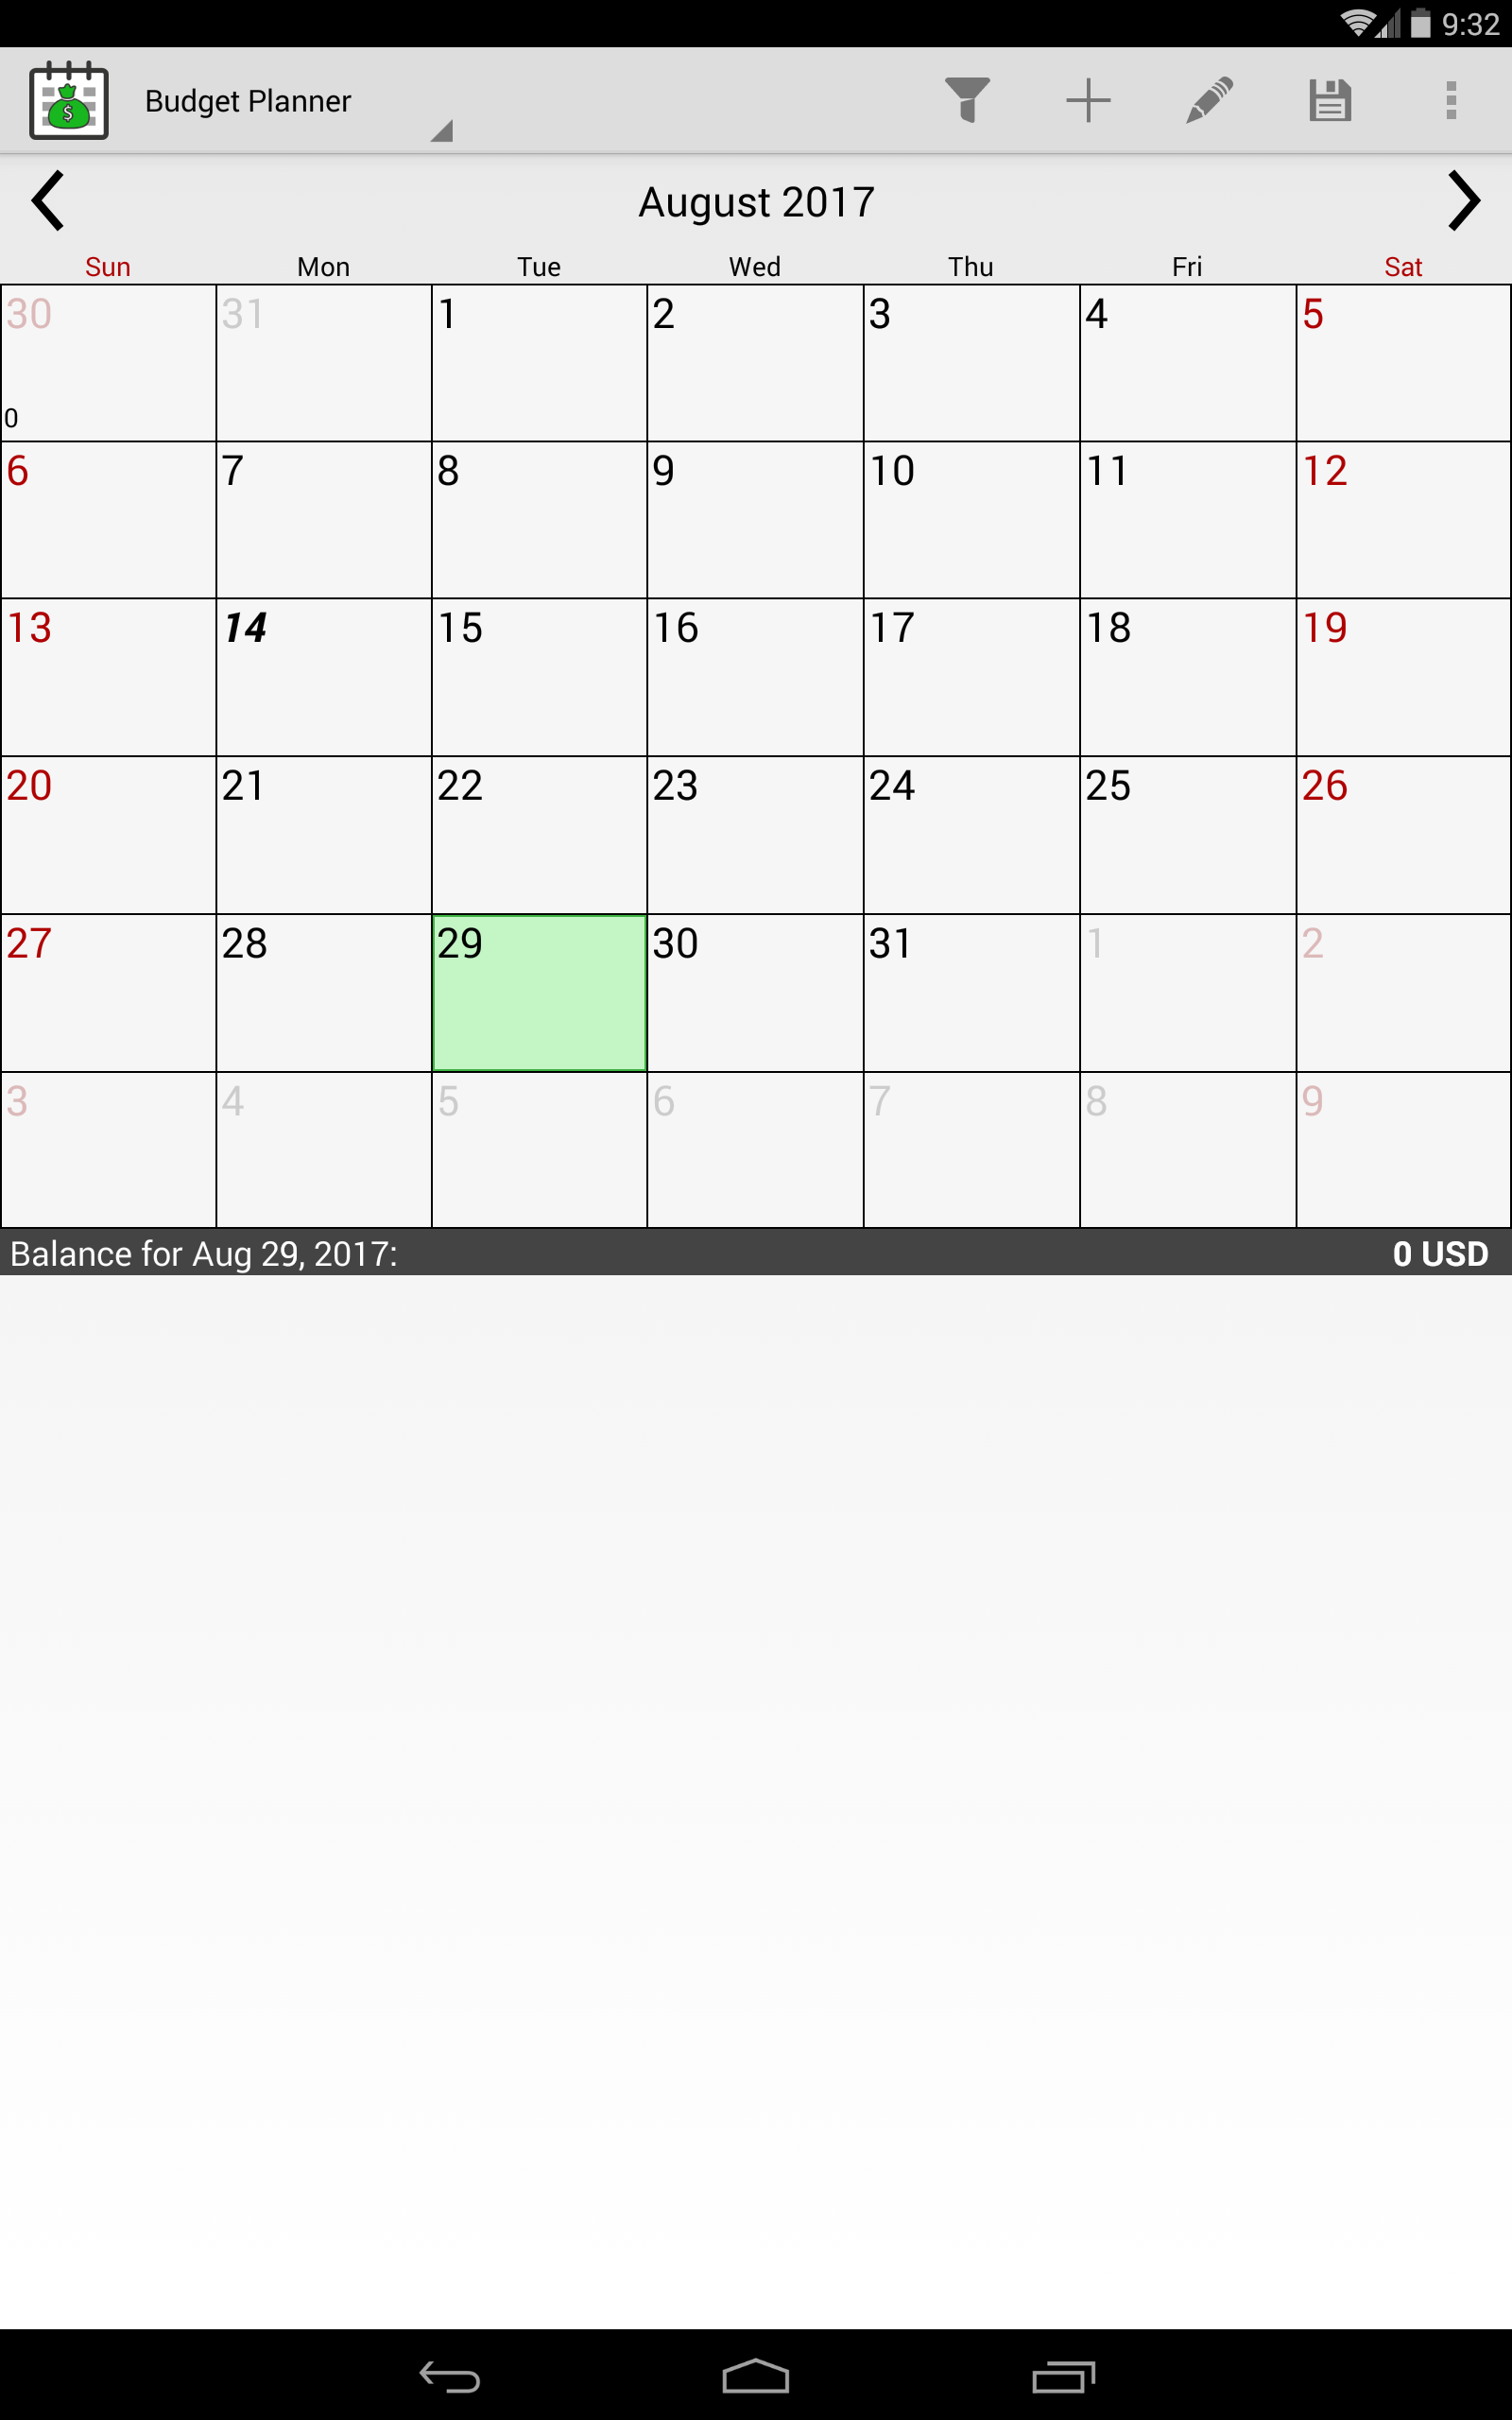
\includegraphics[width=\textwidth]{bp2.png}
		\caption{Budget Planner screenshot-2}
	\end{subfigure}
	\caption{Screenshot captured during analysis}
	\label{fig:bp1}
\end{figure}
\subsubsection{Unique Android SDK API methods}
Number of unique API calls count observed in the run is 4. Following is list of first calls to unique Android SDK API methods:
\begin{itemize}
    \item \texttt{0m 12s - android.telephony.TelephonyManager: java.lang.String getDeviceId()}
\item \texttt{0m 12s - org.apache.http.impl.client.AbstractHttpClient: org.apache.http. HttpResponse (org.apache.http.HttpHost, org.apache.http.protocol.HttpContext)}
\item \texttt{0m 13s - java.net.Socket: void connect (java.net.SocketAddress,int)}
 \item \texttt{0m 13s - android.location.LocationManager: java.lang.String getBestProvider (android.location.Criteria,boolean)}

\end{itemize}
\subsubsection{Unique [API call, event] Android SDK API methods}
Number of unique [API call, event] pairs count observed in the run is 5. Following is the list of first calls to unique Android SDK API methods:
\begin{itemize}
    \item \texttt{0m 12s - reset - android.telephony.TelephonyManager: java.lang.String getDeviceId()}
\item \texttt{0m 12s -  reset - org.apache.http.impl.client.AbstractHttpClient: org.apache. HttpResponse (org.apache.http.HttpHost, org.apache.http.protocol.HttpContext)}
\item \texttt{0m 13s -  reset - java.net.Socket: void connect (java.net.SocketAddress,int)}
\item \texttt{0m 13s -  reset - android.location.LocationManager: java.lang.String.get. BestProvider (android.location.Criteria,boolean)}
\item \texttt{2m 17s - background - android.location.LocationManager:java.lang.String. getBestProvider\\(android.location.Criteria,boolean)}

\end{itemize}
\\
\newline
Figure \ref{fig:bp3} shows the time at which different APIs and (API call, event) pairs are discovered. Total API discovered is 4 and total (API call,event) pair discoverd is 5.
\begin{figure}[!h]
  \centering
  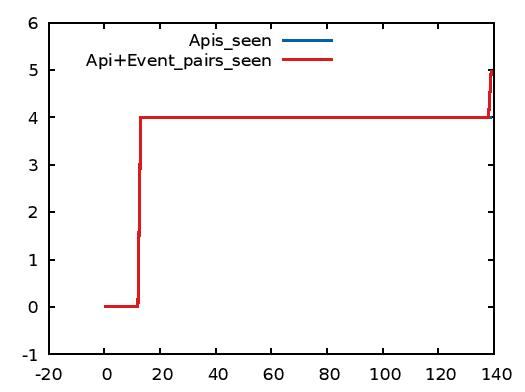
\includegraphics [scale=1.4] {bp3.jpg}
  \caption{API count vs Exploration time}
  \label{fig:bp3}
\end{figure}

\subsubsection{Actionable views}
According Figure \ref{fig:bp4}, nearly 180 unique actionable views is seen and 33 out of 180 views are clicked. The Table \ref{table:1} shows 32 views are clicked once and one views are clicked thrice. 
\begin{figure}[!h]
  \centering
  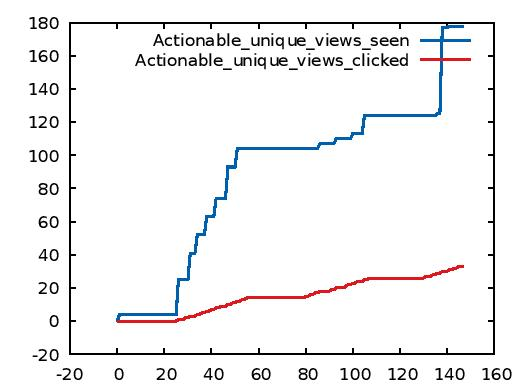
\includegraphics [scale=1.4] {bp4.jpg}
  \caption{API count vs Exploration time}
  \label{fig:bp4}
\end{figure}

\begin{table}[h!]
\centering
\begin{tabular}{||c | c||} 
 \hline
 Number of Click & Views Count \\ [0.5ex] 
 \hline\hline
 0 & 0 \\ 
 1 & 32\\
 2 & 0 \\
 3 & 1\\ [1ex] 

 \hline
\end{tabular}
\caption{Click Frequency of views}

\label{table:1}
\end{table}

\subsubsection{Aggregate stats}
Following is the summary of dynamic analysis of Budget planner application:
\begin{itemize}
    \item File name - budget\_planner-inlined.apk
\item Package name - bdget\_planner
\item Exploration seconds - 153
\item Actions - 39
\item In this reset actions - 3
\item Actionable unique views seen at least once - 178
\item Actionable unique views clicked or long clicked at least once - 33
\item Unique apis - 4
\item Unique event api pairs - 5
\item Exception - N/A (lack of DeviceException)

\end{itemize}

%---------------------------------------------------------------------%
\subsection{BHIM Making India Cashless}
Bharat Interface for Money (BHIM) is an initiative to enable fast, secure, reliable cashless payments through your mobile phone. BHIM is inter operable with other Unified Payment Interface (UPI) applications, & bank accounts for quick money transfers online.
Figure \ref{fig:bhim} shows screenshot taken during the analysis of BHIM applications.
\begin{figure}[!h]
  \centering
  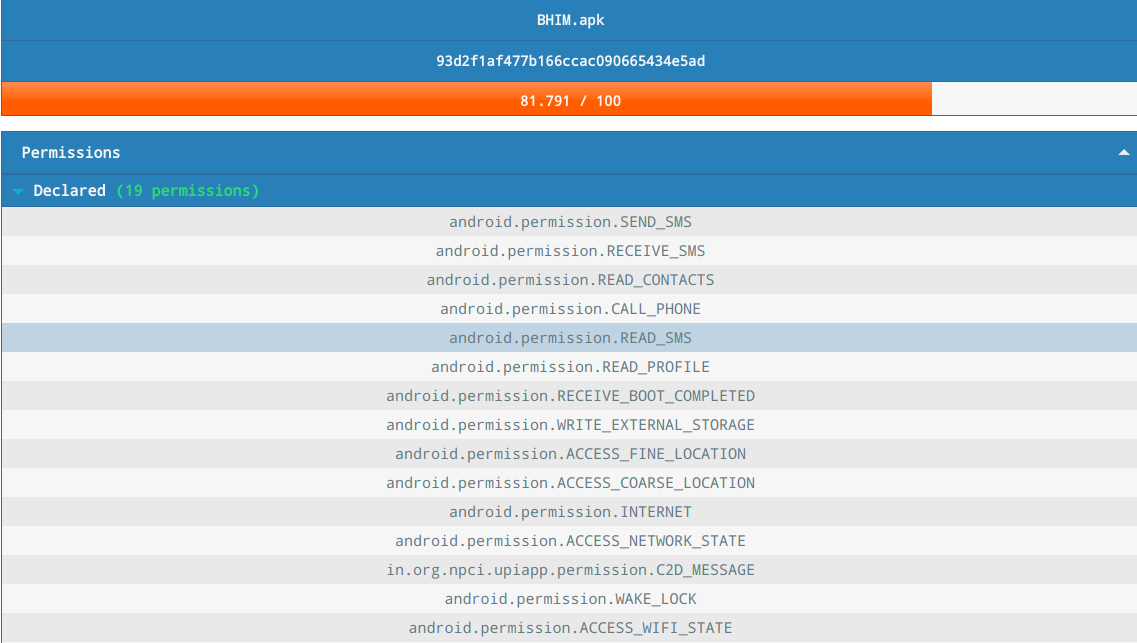
\includegraphics [scale=0.5] {bhim.png}
  \caption{Screenshot captured during analysis of BHIM app}
  \label{fig:bhim}
\end{figure}
\subsubsection{Permissions}
We have extracted the following permissions during the static analysis of BHIM app:\\
\textbf{Required and used} (6 permissions)
\begin{itemize}
    \begin{spacing}{0.9}
    \item \texttt{android.permission.ACCESS\_FINE\_LOCATION} \hfill - Dangerous
    \item \texttt{android.permission.ACCESS\_COARSE\_LOCATION} \hfill - Dangerous
    \item \texttt{android.permission.INTERNET}
    \item \texttt{android.permission.ACCESS\_NETWORK\_STATE}
    \item \texttt{android.permission.WAKE\_LOCK}
    \item \texttt{android.permission.READ\_PHONE\_STATE} \hfill - Dangerous
    \end{spacing}
\end{itemize}
\textbf{Required but not used}(13 permissions)
\begin{itemize}
    \begin{spacing}{0.9}
    \item \texttt{android.permission.SEND\_SMS} \hfill - Dangerous
    \item \texttt{android.permission.RECEIVE\_SMS} \hfill - Dangerous
    \item \texttt{android.permission.READ\_CONTACTS} \hfill - Dangerous
    \item \texttt{android.permission.CALL\_PHONE} \hfill - Dangerous
    \item \texttt{android.permission.READ\_SMS} \hfill - Dangerous
    \item \texttt{android.permission.READ\_PROFILE}
    \item \texttt{android.permission.RECEIVE\_BOOT\_COMPLETED}
    \item \texttt{android.permission.WRITE\_EXTERNAL\_STORAGE} \hfill - Dangerous
    \item \texttt{in.org.npci.upiapp.permission.C2D\_MESSAGE}
    \item \texttt{android.permission.ACCESS\_WIFI\_STATE}
    \item \texttt{android.permission.CAMERA} \hfill - Dangerous
    \item \texttt{android.permission.READ\_EXTERNAL\_STORAGE} \hfill - Dangerous
    \item \texttt{com.google.android.c2dm.permission.RECEIVE}
    \end{spacing}
\end{itemize}
\textbf{Not required but used}(1 permissions)
\begin{itemize}
    \item \texttt{android.permission.VIBRATE}
\end{itemize}

\subsection{Funnyys}
Funnyys is an application which can add charges to your mobile bill by sending costly SMS messages without informing you first. Figure \ref{fig:funnyys} shows screenshot taken during analysis Funnyys app.
\begin{figure}[!h]
  \centering
  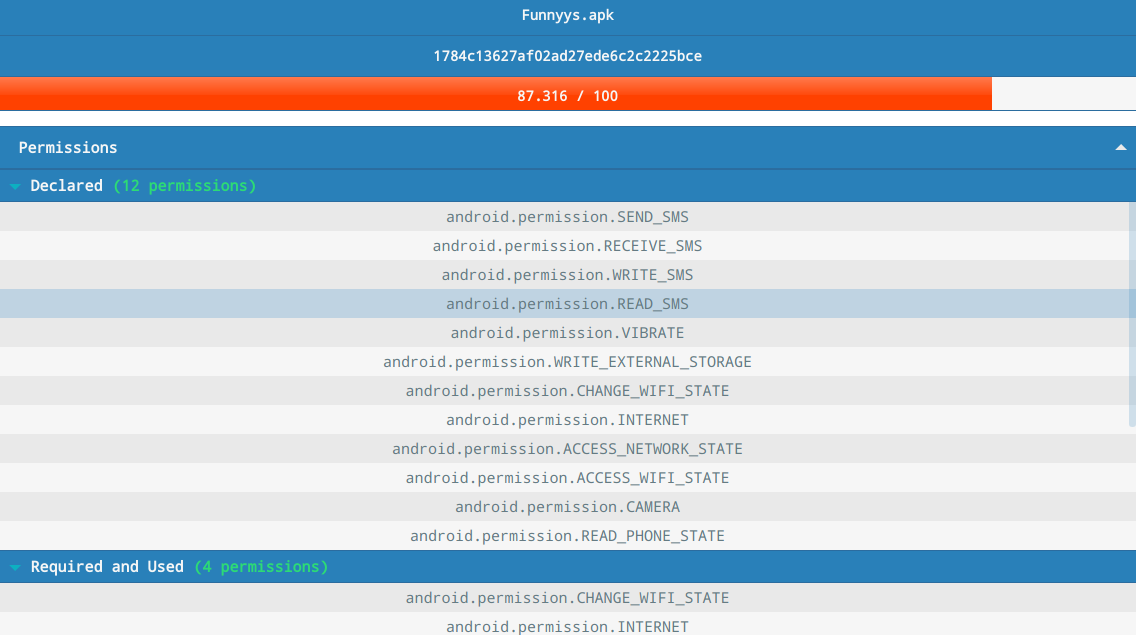
\includegraphics [scale=0.5] {funnyys.png}
  \caption{Screenshot captured during analysis of Funnyys app}
  \label{fig:funnyys}
\end{figure}
\subsubsection{Permissions}
We have extracted the following permissions during the static analysis of Funnyys app:\\
\textbf{Required and used} (4 permissions)
\begin{itemize}
\begin{spacing}{0.9}
\item \texttt{android.permission.CHANGE\_WIFI\_STATE}
\item \texttt{android.permission.INTERNET}
\item \texttt{android.permission.ACCESS\_NETWORK\_STATE}
\item \texttt{android.permission.ACCESS\_WIFI\_STATE}
\end{spacing}
\end{itemize}
\textbf{Required but not used} (8 permissions)
\begin{itemize}
\begin{spacing}{0.9}
\item \texttt{android.permission.SEND\_SMS} \hfill - Dangerous
\item \texttt{android.permission.RECEIVE\_SMS} \hfill - Dangerous
\item \texttt{android.permission.WRITE\_SMS} \hfill - Dangerous
\item \texttt{android.permission.READ\_SMS} \hfill - Dangerous
\item \texttt{android.permission.VIBRATE}
\item \texttt{android.permission.WRITE\_EXTERNAL\_STORAGE} \hfill - Dangerous
\item \texttt{android.permission.CAMERA} \hfill - Dangerous
\item \texttt{android.permission.READ\_PHONE\_STATE} \hfill - Dangerous
\end{spacing}
\end{itemize}
\textbf{Not required but used}(1 permission)
\begin{itemize}
    \item \texttt{android.permission.WAKE\_LOCK}
\end{itemize}
\subsection{Omingo}
This app lets hackers control your device, giving them unauthorized access to your data. Figure \ref{fig:omingo} shows screenshot taken during analysis of Omingo app.
\begin{figure}[!h]
  \centering
  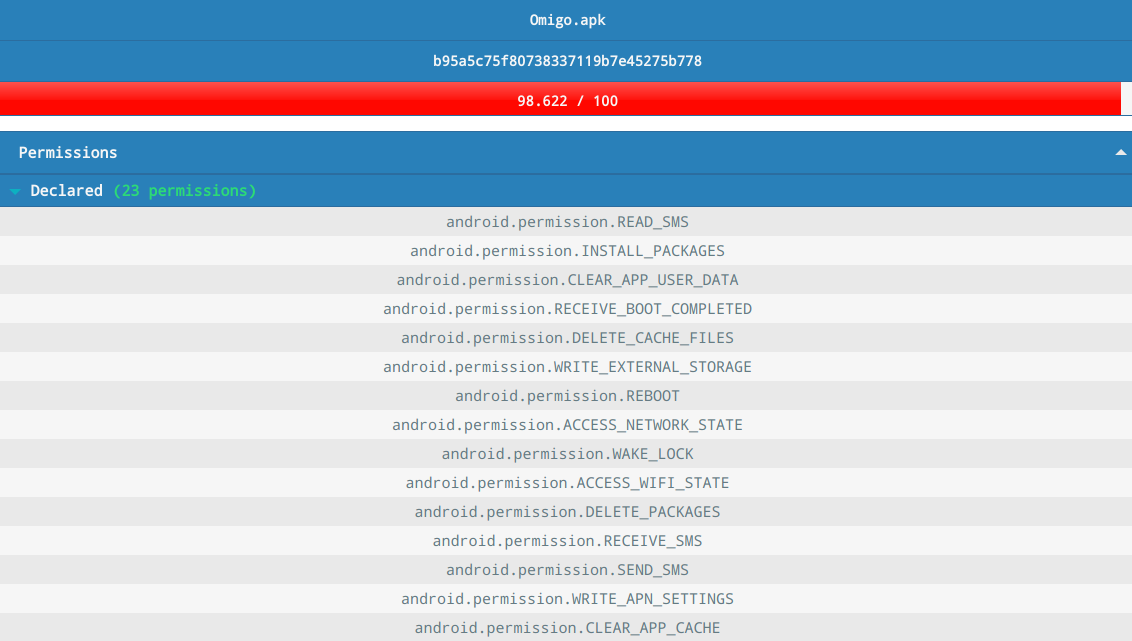
\includegraphics [scale=0.5] {omigo.png}
  \caption{Screenshot captured during analysis of Omingo app}
  \label{fig:omingo}
\end{figure}
\subsubsection{Permissions}
We have extracted the following permissions during the static analysis of Omingo app:\\
\textbf{Required and used} (4 permissions)
\begin{itemize}
\begin{spacing}{0.9}
\item \texttt{android.permission.INTERNET}
\item \texttt{android.permission.ACCESS\_NETWORK\_STATE}
\item \texttt{android.permission.ACCESS\_WIFI\_STATE}
\item \texttt{android.permission.READ\_PHONE\_STATE} \hfill - Dangerous
\end{spacing}
\end{itemize}
\textbf{Required but not used} (19 permissions)
\begin{itemize}
\begin{spacing}{0.9}
\item \texttt{android.permission.RECEIVE\_SMS} \hfill - Dangerous
\item \texttt{android.permission.SEND\_SMS} \hfill - Dangerous
\item \texttt{android.permission.WRITE\_APN\_SETTINGS}
\item \texttt{android.permission.CLEAR\_APP\_CACHE}
\item \texttt{android.permission.READ\_SMS} \hfill - Dangerous
\item \texttt{android.permission.RECEIVE\_WAP\_PUSH}
\item \texttt{android.permission.INSTALL\_PACKAGES} \hfill - Dangerous
\item \texttt{android.permission.CLEAR\_APP\_USER\_DATA}
\item \texttt{android.permission.MOUNT\_UNMOUNT\_FILESYSTEMS}
\item \texttt{android.permission.RECEIVE\_BOOT\_COMPLETED}
\item \texttt{android.permission.DELETE\_CACHE\_FILES}
\item \texttt{android.permission.WRITE\_EXTERNAL\_STORAGE} \hfill - Dangerous
\item \texttt{android.permission.REBOOT} \hfill - Dangerous
\item \texttt{android.permission.RESTART\_PACKAGES} \hfill - Dangerous
\item \texttt{android.permission.CHANGE\_WIFI\_STATE}
\item \texttt{android.permission.WAKE\_LOCK}
\item \texttt{android.permission.CHANGE\_NETWORK\_STATE}
\item \texttt{android.permission.SET\_WALLPAPER}
\item \texttt{android.permission.DELETE\_PACKAGES} \hfill - Dangerous
\end{spacing}
\end{itemize}
\textbf{Not required but used}(3 permission)
\begin{itemize}
\begin{spacing}{0.9}
\item \texttt{android.permission.ACCESS\_FINE\_LOCATION} \hfill - Dangerous
\item \texttt{android.permission.ACCESS\_COARSE\_LOCATION} \hfill - Dangerous
\item \texttt{android.permission.VIBRATE}
\end{spacing}
\end{itemize}
\subsection{System Certificate}
System Certificate  is a fake application which can damage your device and steal your data. Figure \ref{fig:system} shows the screenshot taken during static analysis of System Certificate app.
\begin{figure}[!h]
  \centering
  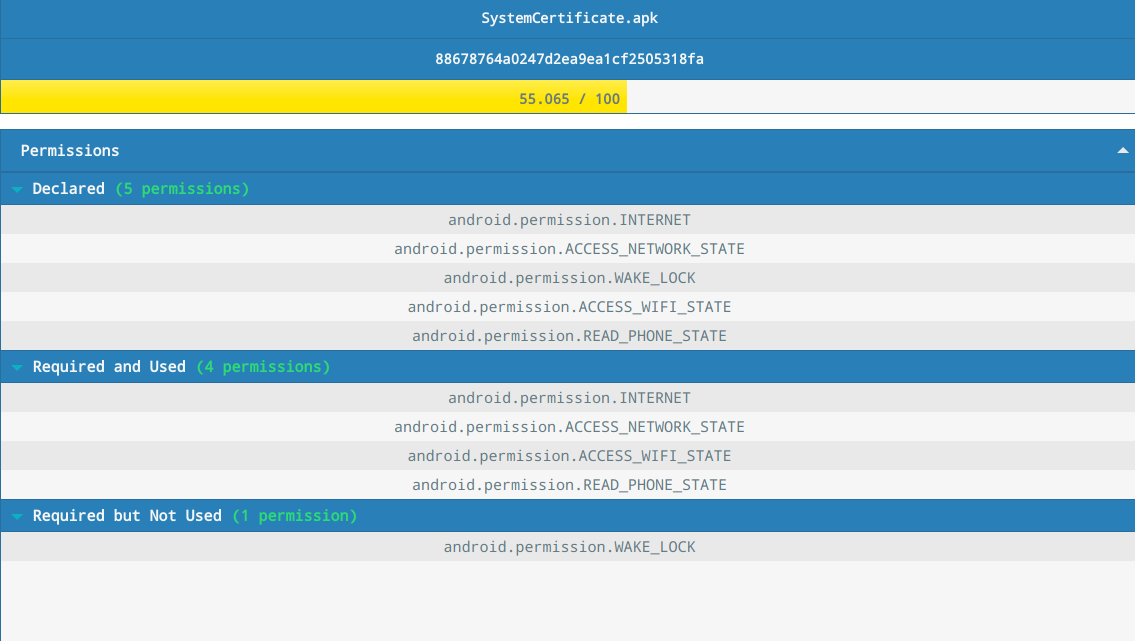
\includegraphics [scale=0.5] {system.png}
  \caption{Screenshot captured during analysis of System Certificate app}
  \label{fig:system}
\end{figure}
\subsubsection{Permissions}
We have extracted the following permissions during the static analysis of System Certificate app:\\

\textbf{Required and used} (4 permissions)
\begin{itemize}
\begin{spacing}{0.9}
\item \texttt{android.permission.INTERNET}
\item \texttt{android.permission.ACCESS\_NETWORK\_STATE}
\item \texttt{android.permission.ACCESS\_WIFI\_STATE}
\item \texttt{android.permission.READ\_PHONE\_STATE} \hfill - Dangerous
\end{spacing}
\end{itemize}
\textbf{Required but not used} (1 permissions)
\begin{itemize}
    \item \texttt{android.permission.WAKE\_LOCK}
\end{itemize}

\subsection{Tez – A new payments app by Google}
Tez is an application send money to others. It is developed by Google. It is based on UPI. Figure \ref{fig:tez} shows the screenshot taken during the analysis Tez app.
\begin{figure}[!h]
  \centering
  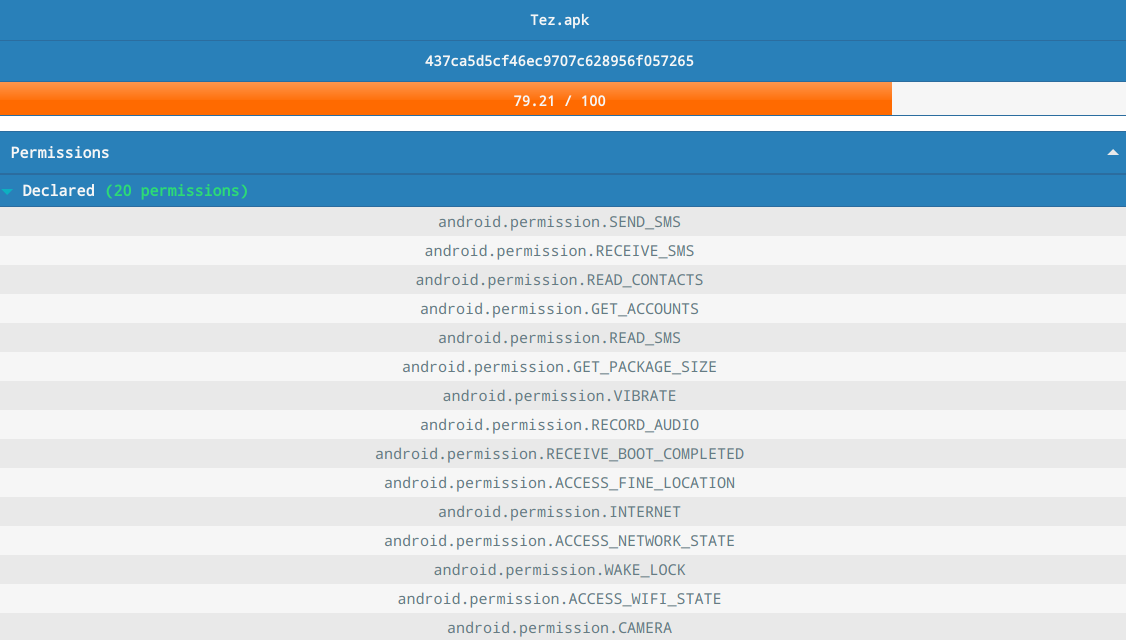
\includegraphics [scale=0.5] {tez.png}
  \caption{Screenshot captured during analysis of Tez app}
  \label{fig:tez}
\end{figure}
\subsubsection{Permissions}
We have extracted the following permissions during the static analysis of Tez app:\\
\textbf{Required and used} (6 permissions)
\begin{itemize}
\begin{spacing}{0.9}
\item \texttt{android.permission.INTERNET}
\item \texttt{android.permission.VIBRATE}
\item \texttt{android.permission.ACCESS\_NETWORK\_STATE}
\item \texttt{android.permission.WAKE\_LOCK}
\item \texttt{android.permission.BLUETOOTH}
\item \texttt{android.permission.READ\_PHONE\_STATE} \hfill - Dangerous
\end{spacing}
\end{itemize}
\textbf{Required but not used} (14 permissions)
\begin{itemize}
\begin{spacing}{0.9}
\item \texttt{android.permission.SEND\_SMS} \hfill - Dangerous
\item \texttt{android.permission.RECEIVE\_SMS} \hfill - Dangerous
\item \texttt{android.permission.READ\_CONTACTS} \hfill - Dangerous
\item \texttt{android.permission.GET\_ACCOUNTS} \hfill - Dangerous
\item \texttt{android.permission.READ\_SMS} \hfill - Dangerous
\item \texttt{android.permission.GET\_PACKAGE\_SIZE}
\item \texttt{android.permission.RECORD\_AUDIO} \hfill - Dangerous
\item \texttt{android.permission.RECEIVE\_BOOT\_COMPLETED}
\item \texttt{android.permission.ACCESS\_FINE\_LOCATION} \hfill - Dangerous
\item \texttt{android.permission.ACCESS\_WIFI\_STATE}
\item \texttt{android.permission.CAMERA} \hfill - Dangerous
\item \texttt{android.permission.MANAGE\_ACCOUNTS} \hfill - Dangerous
\item \texttt{com.google.android.c2dm.permission.RECEIVE}
\item \texttt{com.google.android.providers.gsf.permission.READ\_GSERVICES}
\end{spacing}
\end{itemize}
\textbf{Not required but used} (2 permission)
\begin{itemize}
\item \texttt{android.permission.ACCESS\_COARSE\_LOCATION} \hfill - Dangerous
\item \texttt{android.permission.MODIFY\_AUDIO\_SETTINGS}
\end{itemize}
\subsection{MMS Beline}
MMS Beline is an application which can call phone number  and also send SMS without informing you, which will lead to increase in mobile bill. This application can steal your data and can run with administrative permissions. Figure \ref{fig:mms} shows the screenshot taken during the static analysis of MMS Beline.
\begin{figure}[!h]
  \centering
  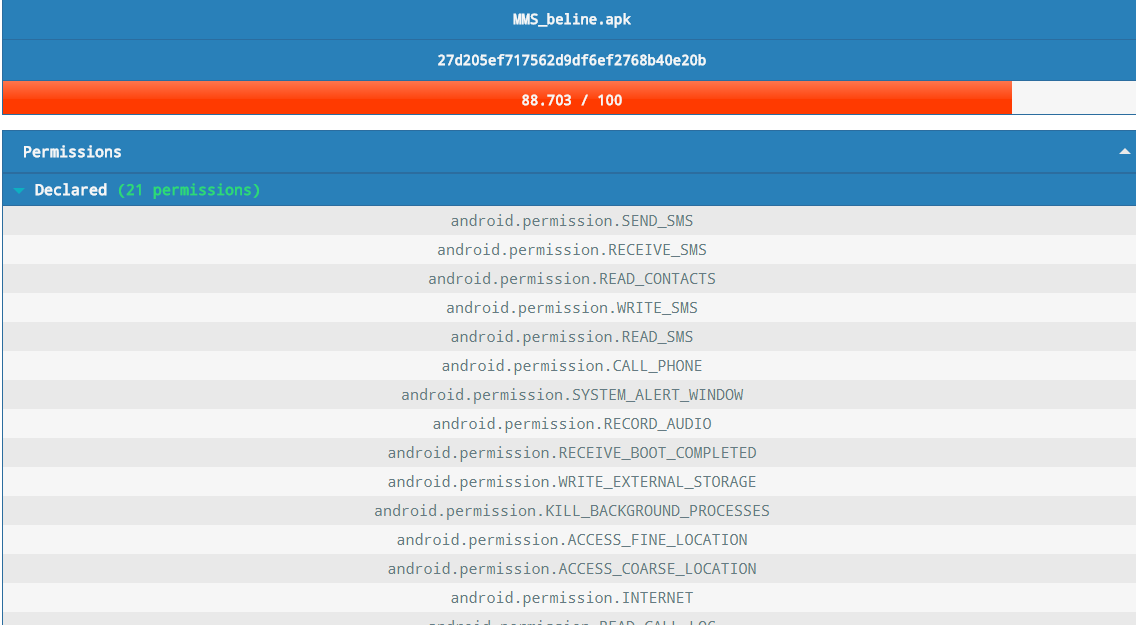
\includegraphics [scale=0.5] {mms.png}
  \caption{Screenshot captured during analysis of MMS Beline app}
  \label{fig:mms}
\end{figure}
\subsubsection{Permissions}
We have extracted the following permissions during the static analysis of MMS beline app:\\
\textbf{Required and used} (5 permissions)
\begin{itemize}
\begin{spacing}{0.9}
\item \texttt{android.permission.ACCESS\_FINE\_LOCATION} \hfill - Dangerous
\item \texttt{android.permission.ACCESS\_COARSE\_LOCATION} \hfill - Dangerous
\item \texttt{android.permission.INTERNET}
\item \texttt{android.permission.GET\_TASKS}
\item \texttt{android.permission.READ\_PHONE\_STATE} \hfill - Dangerous
\end{spacing}
\end{itemize}
\textbf{Required but not used} (16 permissions)
\begin{itemize}
\begin{spacing}{0.9}
\item \texttt{android.permission.SEND\_SMS} \hfill - Dangerous
\item \texttt{android.permission.RECEIVE\_SMS} \hfill - Dangerous
\item \texttt{android.permission.READ\_CONTACTS} \hfill - Dangerous
\item \texttt{android.permission.WRITE\_SMS} \hfill - Dangerous
\item \texttt{android.permission.READ\_SMS} \hfill - Dangerous
\item \texttt{android.permission.CALL\_PHONE} \hfill - Dangerous
\item \texttt{android.permission.SYSTEM\_ALERT\_WINDOW}
\item \texttt{android.permission.RECORD\_AUDIO} \hfill - Dangerous
\item \texttt{android.permission.RECEIVE\_BOOT\_COMPLETED}
\item \texttt{android.permission.WRITE\_EXTERNAL\_STORAGE} \hfill - Dangerous
\item \texttt{android.permission.KILL\_BACKGROUND\_PROCESSES} \hfill - Dangerous
\item \texttt{android.permission.READ\_CALL\_LOG} \hfill - Dangerous
\item \texttt{android.permission.ACCESS\_NETWORK\_STATE}
\item \texttt{android.permission.WAKE\_LOCK}
\item \texttt{android.permission.CAMERA} \hfill - Dangerous
\item \texttt{android.permission.READ\_EXTERNAL\_STORAGE} \hfill - Dangerous
\end{spacing}
\end{itemize}
\subsection{Google Calendar}
Google Calendar is the free time management web application offered by Google.Google Calendar allows users to create and edit events. Reminders can be enabled for events, with options available for type and time. Event locations can also be added, and other users can be invited to events. Users can enable or disable the visibility of special calendars, including Birthdays, where the app retrieves dates of births from Google contacts and displays birthday cards on a yearly basis, and Holidays, a country-specific calendar that displays dates of special occasions. Figure \ref{fig:cal} shows the screenshot taken during the static analysis of Calendar app.
\begin{figure}[!h]
  \centering
  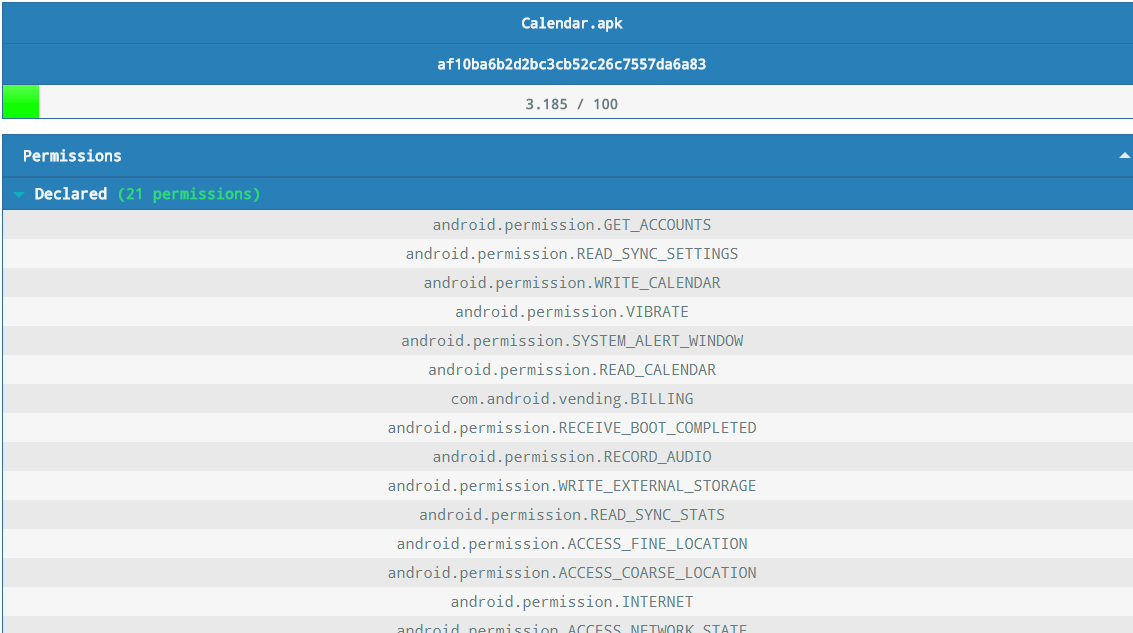
\includegraphics [scale=0.5] {cal.png}
  \caption{Screenshot captured during analysis}
  \label{fig:cal}
\end{figure}
\subsubsection{Permissions}
We have extracted the following permissions during the static analysis of Calendar app:\\
\textbf{Required and used} (8 permissions)
\begin{itemize}
\begin{spacing}{0.9}
\item \texttt{android.permission.ACCESS\_FINE\_LOCATION} \hfill - Dangerous
\item \texttt{android.permission.ACCESS\_COARSE\_LOCATION} \hfill - Dangerous
\item \texttt{android.permission.INTERNET}
\item \texttt{android.permission.VIBRATE}
\item \texttt{android.permission.ACCESS\_NETWORK\_STATE}
\item \texttt{android.permission.WAKE\_LOCK}
\item \texttt{android.permission.RECORD\_AUDIO} \hfill - Dangerous
\item \texttt{android.permission.WRITE\_EXTERNAL\_STORAGE} \hfill - Dangerous
\end{spacing}
\end{itemize}
\textbf{Required but not used} (13 permissions)
\begin{itemize}
\begin{spacing}{0.9}
\item \texttt{android.permission.GET\_ACCOUNTS} \hfill - Dangerous
\item \texttt{android.permission.READ\_SYNC\_SETTINGS}
\item \texttt{android.permission.WRITE\_CALENDAR} \hfill - Dangerous
\item \texttt{android.permission.SYSTEM\_ALERT\_WINDOW}
\item \texttt{android.permission.READ\_CALENDAR} \hfill - Dangerous
\item \texttt{com.android.vending.BILLING}
\item \texttt{android.permission.RECEIVE\_BOOT\_COMPLETED}
\item \texttt{android.permission.READ\_SYNC\_STATS}
\item \texttt{android.permission.GET\_TASKS}
\item \texttt{android.permission.READ\_EXTERNAL\_STORAGE} \hfill - Dangerous
\item \texttt{android.permission.WRITE\_SETTINGS}
\item \texttt{android.permission.READ\_PHONE\_STATE}
\item \texttt{com.google.android.providers.gsf.permission.READ\_GSERVICES}
\end{spacing}
\end{itemize}
\subsubsection{Unique Android SDK API methods}
Number of unique API calls count observed in the run is 4. Following is list of first calls to unique Android SDK API methods:
\begin{itemize}
    \item \texttt{0m 12s  - android.app.ActivityThread: void installContentProviders (android. content.Context, java.util.List)}
  \item \texttt{0m 12s  -  android.content.ContentResolver: android.database.Cursor query (android.net.Uri, java.lang.String[], java.lang.String, java.lang.String[], java.lang.String,android.os. CancellationSignal)}
 \item  \texttt{0m 12s  -  android.content.ContentResolver: android.database. Cursor query (android.net.Uri, java.lang.String[], java.lang.String,java.lang.String[],  java.lang.String, android.os. CancellationSignal)}
\item   \texttt{0m 12s  -  android.content.ContentResolver: android.database.Cursor query ( android.net.Uri, java.lang.String[], java.lang.String, java.lang.String[], java.lang.String,android.os. CancellationSignal)}
\item   \texttt{0m 12s  -  android.content.ContentResolver:void registerContentObserver( android.net.Uri, boolean ,android.database.ContentObserver, int)}
\item   \texttt{0m 12s -  android.content.ContentResolver: void registerContentObserver (android.net.Uri, boolean, android.database.ContentObserver, int)}
  \item \texttt{0m 12s  -  android.content.ContentResolver: android.database.Cursor query (android.net.Uri, java.lang.String[], java.lang.String, java.lang.String[], java.lang.String, android.os. CancellationSignal)}
 \item  \texttt{0m 12s  -  android.content.ContentResolver: android.database.Cursor query (android.net.Uri, java.lang.String[], java.lang.String, java.lang.String[],  java.lang.String,android.os. CancellationSignal)}
 \item  \texttt{0m 24s  -  android.content.ContentResolver: android.database.Cursor query (android.net.Uri, java.lang.String[], java.lang.String,java.lang.String[],  java.lang.String,android.os. CancellationSignal)}
 \item  \texttt{0m 27s  -  android.content.ContentResolver: android.database.Cursor query (android.net.Uri, java.lang.String[], java.lang.String,java.lang.String[], java.lang.String,android.os. CancellationSignal)}
 \item  \texttt{0m 31s  -  android.content.ContentResolver: android.database.Cursor query  (android.net.Uri, java.lang.String[], java. lang.String,java.lang.String[], j ava.lang.String,android.os. CancellationSignal)}
  \item \texttt{0m 33s  -  android.content.ContentResolver: android.database.Cursor query (android.net.Uri, java.lang.String[], java.lang.String, java.lang.String[], java.lang.String, android.os. CancellationSignal)}
 \item  \texttt{0m 38s  -  android.content.ContentResolver: android.database. Cursor query (android.net.Uri, java.lang.String[], java.lang.String, java.lang.String[],  java.lang.String,android. os.CancellationSignal)}
\item   \texttt{0m 38s  -  android.content.ContentResolver: void registerContentObserver (android.net.Uri, boolean, android.database.ContentObserver, int)}
 \item  \texttt{1m 21s  -  android.content.ContentResolver: android.database.Cursor query (android.net.Uri, java.lang.String[], java.lang.String, java.lang.String[], java.lang.String, android.os. CancellationSignal)}
 \item  \texttt{1m 23s  -  android.content.ContentResolver: android.database.Cursor query (android.net.Uri, java.lang.String[], java.lang.String, java.lang.String[], java.lang.String,android.os. CancellationSignal)}
 \item  \texttt{1m 54s  -  android.content.ContentResolver: android.database.Cursor query (android.net.Uri, java.lang.String[], java.lang.String, java.lang.String[], java.lang.String, android.os. CancellationSignal)}
 \item  \texttt{1m 56s  -  android.content.ContentResolver: android.database.Cursor query (android.net.Uri, java.lang.String[], java.lang.String, java.lang.String[], java.lang.String, android.os. CancellationSignal)}
 \item  \texttt{2m 11s   -  android.content.ContentResolver: android.database.Cursor query (android.net.Uri, java.lang.String[], java.lang.String, java.lang.String[],  java.lang.String, android.os. CancellationSignal)}

\end{itemize}

Figure \ref{fig:cal_api} shows the time at which different APIs and (API call, event) pairs are discovered. Total API discovered is 4 and total (API call,event) pair discovered is 5.
\begin{figure}[!h]
  \centering
  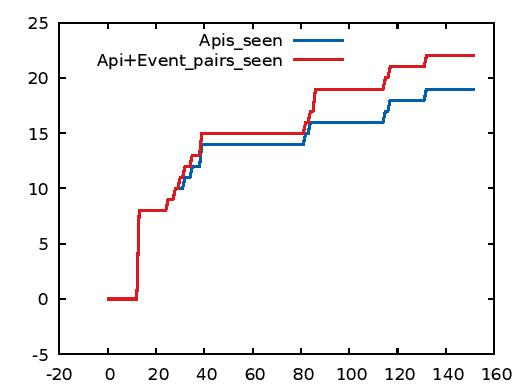
\includegraphics [scale=1.4] {cal_api.jpg}
  \caption{API count vs Exploration time}
  \label{fig:cal_api}
\end{figure}

\subsubsection{Actionable views}
According Figure \ref{fig:cal_view}, nearly 180 unique actionable views is seen and 33 out of 180 views are clicked. The Table \ref{table:2} shows 18 views are clicked once and 6 views are clicked twice. 
\begin{figure}[!h]
  \centering
  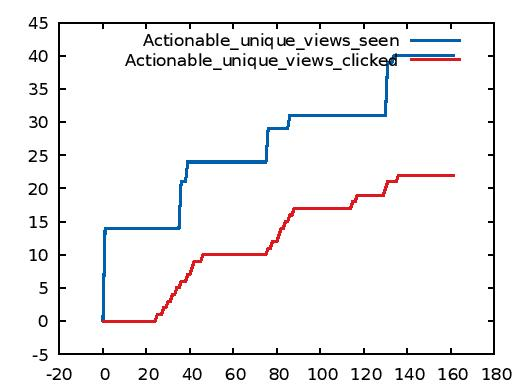
\includegraphics [scale=1.4] {cal_view.jpg}
  \caption{API count vs Exploration time}
  \label{fig:cal_view}
\end{figure}

\begin{table}[h!]
\centering
\begin{tabular}{||c | c||} 
 \hline
 Number of Click & Views Count \\ [0.5ex] 
 \hline\hline
 0 & 0 \\ 
 1 & 18\\
 2 & 6\\ [1ex] 

 \hline
\end{tabular}
\caption{Click Frequency of views}

\label{table:2}
\end{table}

\subsubsection{Aggregate stats}
Following is the summary of dynamic analysis of Google Calendar application:
\begin{itemize}
\begin{spacing}{1.2}
\item File name - Calendar-inlined.apk
\item Package name - com.google.android.calendar
\item Exploration seconds - 167
\item Actions - 35
\item In this reset actions - 4
\item Actionable unique views seen at least once - 40
\item Actionable unique views clicked or long clicked at least once - 22
\item Unique apis - 19
\item Unique event api pairs - 22
\item Exception - N/A (lack of DeviceException)
\end{spacing}
\end{itemize}

%---------------------------------------------------------------------%

%---------------------------------------------------------------------%


%---------------------------------------------------------------------%
%---------------------------------------------------------------------%
%------------------------------------------------------------------------------%
\subsection{Laughtter}
Laughtter is an application which can add charges to your mobile bill by sending costly SMS message without informing you first. Figure \ref{fig:laughtter} shows the screenshot taken during analysis of Laughtter app.
\begin{figure}[!h]
  \centering
  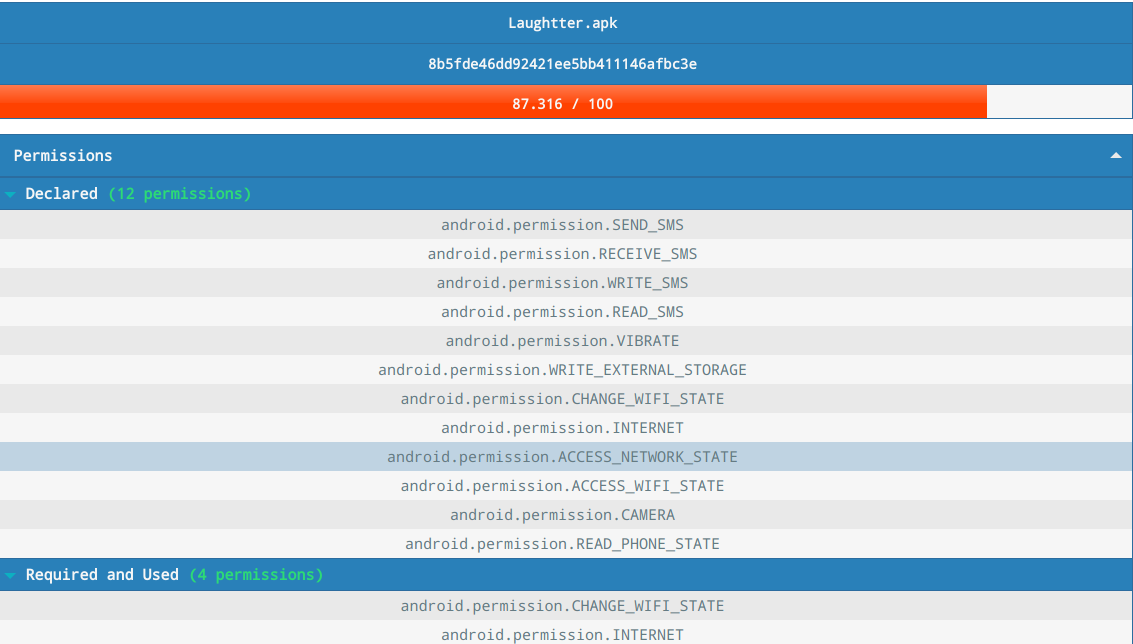
\includegraphics [scale=0.5] {laughtter.png}
  \caption{Screenshot captured during analysis of Laughtter app}
  \label{fig:laughtter}
\end{figure}
\subsubsection{Permissions}
We have extracted the following permissions during the static analysis of Laughtter app:\\
\textbf{Required and used} (4 permissions)
\begin{itemize}
\begin{spacing}{0.9}
\item \texttt{android.permission.CHANGE\_WIFI\_STATE}
\item \texttt{android.permission.INTERNET}
\item \texttt{android.permission.ACCESS\_NETWORK\_STATE}
\item \texttt{android.permission.ACCESS\_WIFI\_STATE}
\end{spacing}
\end{itemize}
\textbf{Required but not used} (8 permissions)
\begin{itemize}
\begin{spacing}{0.9}
\item \texttt{android.permission.SEND\_SMS} \hfill - Dangerous
\item \texttt{android.permission.RECEIVE\_SMS} \hfill - Dangerous
\item \texttt{android.permission.WRITE\_SMS} \hfill - Dangerous
\item \texttt{android.permission.READ\_SMS} \hfill - Dangerous
\item \texttt{android.permission.VIBRATE}
\item \texttt{android.permission.WRITE\_EXTERNAL\_STORAGE} \hfill - Dangerous
\item \texttt{android.permission.CAMERA} \hfill - Dangerous
\item \texttt{android.permission.READ\_PHONE\_STATE} \hfill - Dangerous
\end{spacing}
\end{itemize}
\textbf{Not required but used} (1 permissions)
\begin{itemize}
    \item \texttt{android.permission.WAKE\_LOCK}
\end{itemize}

\subsection{Android Framework}
Android Framework lets control your device, giving them unauthorized access to your data. Figure \ref{fig:andro} shows the screenshot taken during static analysis of the application.
\begin{figure}[!h]
  \centering
  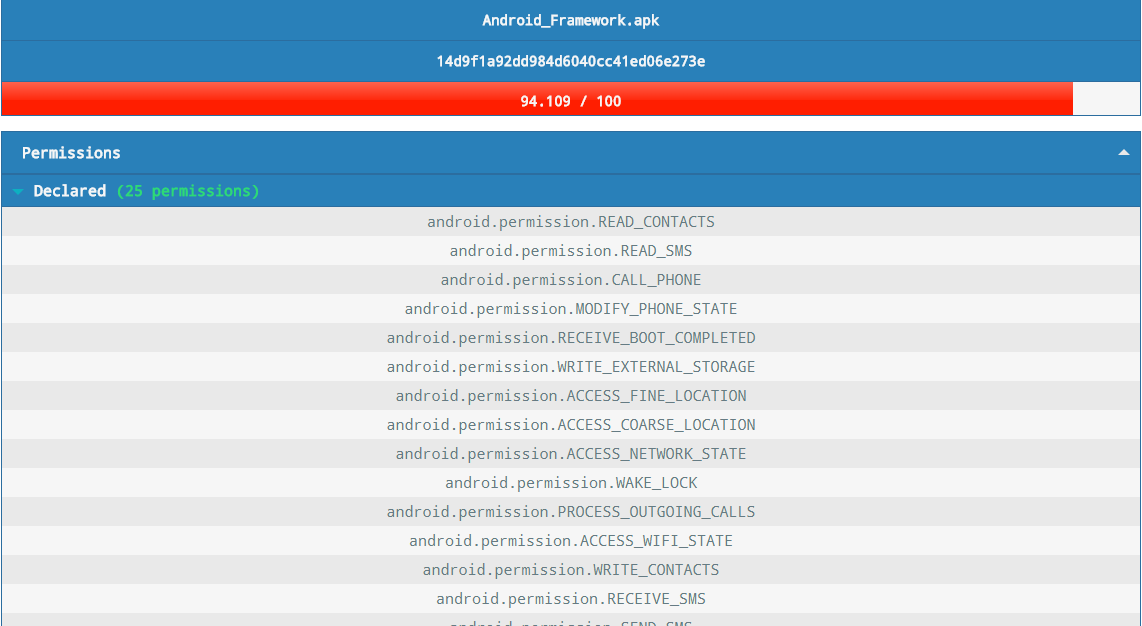
\includegraphics [scale=0.5] {andro.png}
  \caption{Screenshot captured during analysis of Android Framework app}
  \label{fig:andro}
\end{figure}
\subsubsection{Permissions}
We have extracted following permissions during the analysis of Android Framework application:\\
\textbf{Requested and used} (9 permissions)
\begin{itemize}
\begin{spacing}{0.9}    
\item \texttt{android.permission.ACCESS\_FINE\_LOCATION} \hfill - Dangerous
\item \texttt{android.permission.ACCESS\_COARSE\_LOCATION} \hfill - Dangerous
\item \texttt{android.permission.CHANGE\_WIFI\_STATE}
\item \texttt{android.permission.INTERNET}
\item \texttt{android.permission.ACCESS\_NETWORK\_STATE}
\item \texttt{android.permission.WAKE\_LOCK}
\item \texttt{android.permission.ACCESS\_WIFI\_STATE}
\item \texttt{android.permission.RECORD\_AUDIO} \hfill - Dangerous
\item \texttt{android.permission.READ\_PHONE\_STATE} \hfill - Dangerous
\end{spacing}
\end{itemize}
\textbf{Requested but not used} (16 permissions)
\begin{itemize}
\begin{spacing}{0.9}
\item \texttt{android.permission.READ\_CONTACTS} \hfill - Dangerous
\item \texttt{android.permission.READ\_SMS} \hfill - Dangerous
\item \texttt{android.permission.CALL\_PHONE} \hfill - Dangerous
\item \texttt{android.permission.MODIFY\_PHONE\_STATE} \hfill - Dangerous
\item \texttt{android.permission.RECEIVE\_BOOT\_COMPLETED}
\item \texttt{android.permission.WRITE\_EXTERNAL\_STORAGE} \hfill - Dangerous
\item \texttt{android.permission.PROCESS\_OUTGOING\_CALLS} \hfill - Dangerous
\item \texttt{android.permission.WRITE\_CONTACTS} \hfill - Dangerous
\item \texttt{android.permission.RECEIVE\_SMS} \hfill - Dangerous
\item \texttt{android.permission.SEND\_SMS} \hfill - Dangerous
\item \texttt{android.permission.WRITE\_APN\_SETTINGS}
\item \texttt{android.permission.WRITE\_SMS} \hfill - Dangerous
\item \texttt{android.permission.BROADCAST\_PACKAGE\_REMOVED}
\item \texttt{android.permission.CHANGE\_NETWORK\_STATE}
\item \texttt{android.permission.MODIFY\_AUDIO\_SETTINGS}
\item \texttt{android.permission.READ\_EXTERNAL\_STORAGE} \hfill - Dangerous
\end{spacing}
\end{itemize}



% Main chapter title
\chapter{App Classification Models}
\label{ch:proposed}

% This is for the header on each page
\lhead{Chapter 5. \emph{App Classification Models}}
\thispagestyle{empty}
Classification is the technique to classify new observation on the basis of a set of data containing observations whose class is known \cite{wiki:xxx}. Classification is considered as an instance of supervised learning i.e. learning where training set of correctly identified observation is available. To build a classification model we need labelled data. We train classification model with using machine learning algorithm. Figure \ref{fig:appc1} shows the workflow of building the model. Once the model is trained, we feed new observation into classification model to classify them. Figure \ref{fig:appc2} shows the architecture of classifying the new observation using trained Model.
\begin{figure}[!h]
  \centering
  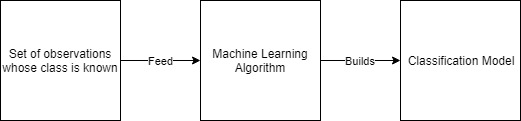
\includegraphics [scale=0.8] {appc1.jpg}
  \caption{Workflow of building a classification model.}
  \label{fig:appc1}
\end{figure}

\begin{figure}[!h]
  \centering
  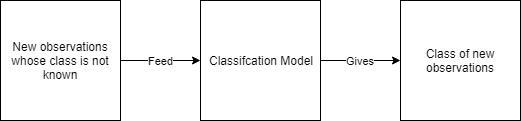
\includegraphics [scale=0.8] {appc2.jpg}
  \caption{Workflow of classifying the new observations.}
  \label{fig:appc2}
\end{figure}
To check the performance of model we have used confusion matrix \cite{wiki:xxx1}. A confusion matrix is a summary of prediction results on a classification problem. The number of correct and incorrect predictions are summarized with count values and broken down by each class. The confusion matrix shows the ways in which your classification model is confused when it makes predictions. It gives us insight not only into the errors being made by a classifier but more importantly the types of errors that are being made. A classification model is good if there is high value along the diagonal of confusion matrix. Table \ref{table:tab1} shows the general confusion matrix.\\
\begin{table}[!h]
\centering

\begin{tabular}{|l||l|l|}
\hline
\multirow{2}{4em}{Actual} & \multicolumn{2}{l|}{Predicted} \\ \cline{2-3} 
                  &    Benign      &    Malicious       \\ \hline
         Benign         &      TB     &     FM      \\ \hline
         Malicious          &     FB      &      TM     \\ \hline
\end{tabular}%

\caption{Confusion Matrix}
\label{table:tab1}
\end{table}\\
\textbf{Definition of the Terms: }
\begin{itemize}
    \item Benign (B): Observation is benign.
    \item Malicious (M): Observation is malicious.
    \item True Benign (TB): Observation is benign, and is predicted to be benign.
    \item False Malicious (FM): Observation is benign, but is predicted malicious.
    \item True Malicious (TM): Observation is malicious, and is predicted to be malicious.
    \item False Benign (FM): Observation is malicious, but is predicted benign.
\end{itemize}

We have collected the labelled data of 26000+ applications \cite{dataforclassmodel}.
Data set contains observations/traces of 25593 benign applications and 741 malicious applications. API calls has been used as the feature vector for application. Each application has 854 features. We have developed various classification models using machine learning techniques to classify new applications as benign or malicious. We have used following machine learning techniques:
\begin{enumerate}
    \item Logistic Regression
    \item Support Vector Machine
    \item Neural Network
    \item Random Forest
\end{enumerate} 

\section{Logistic Regression}
Logistic Regression is a classification technique which is is usually taken to apply to a binary dependent variable \cite{wiki:xxx2}. We have divided the data set into training set which is 80\% of the total data set and testing set which 20\% of the total data set. We have trained our model on the training set and have checked the performance of the model on test data. Model classifies 93.8\% of benign correctly and 83.4\% of malicious app correctly. Table \ref{table:tab2} shows the confusion matrix obtained from Logistic regression model. 
\begin{table}[!h]
\centering

\begin{tabular}{|l||l|l|}
\hline
\multirow{2}{4em}{Actual} & \multicolumn{2}{l|}{Predicted} \\ \cline{2-3} 
                  &    benign      &    malicious       \\ \hline
         benign         &      93.8     &    6.2       \\ \hline
        malicious          &     16.6      &      83.4     \\ \hline
\end{tabular}%
\caption{Confusion matrix for Logistic regression}
\label{table:tab2}
\end{table}
We have used this model to predict the class of applications which we have analyzed. Following application is classified as benign:
\begin{itemize}
    \item Budget Planner
    \item BHIM Making India Cashless
    \item System Certificate
    \item Tez: A new payment app by Google
    \item Google Calendar
\end{itemize}
Following application is classified as malicious:
\begin{itemize}
    \item Funnyys
    \item Omingo
    \item MMS Beline
    \item Laughtter
    \item Android Framework
\end{itemize}

\section{Support Vector Machine}
In machine learning, Support Vector Machine (SVM) is considered as supervised learning models associated with learning algorithms \cite{wiki:xxx3}. Here, we have used this model for classification. We have divided the data set into training set which is 80\% of the total data set and testing set which 20\% of the total data set. We have trained our model on the training set and have checked the performance of the model on test data. Model classifies 92.6\% of benign correctly and 78.7\% of malicious app correctly. Table \ref{table:tab3} shows the confusion matrix obtained from Support Vector Machine model.
\begin{table}[!h]
\centering

\begin{tabular}{|l||l|l|}
\hline
\multirow{2}{4em}{Actual} & \multicolumn{2}{l|}{Predicted} \\ \cline{2-3} 
                  &    benign      &    malicious       \\ \hline
         benign         &      92.6     &    7.4      \\ \hline
        malicious          &     21.3      &      78.7     \\ \hline
\end{tabular}%
\caption{Confusion matrix for Support Vector Machine}
\label{table:tab3}
\end{table}
We have used this model to predict the class of applications which we have analyzed. Following application is classified as benign:
\begin{itemize}
    \item Budget Planner
    \item Funnyys
    \item BHIM Making India Cashless
    \item System Certificate
    \item Tez: A new payment app by Google
    \item Google Calendar
\end{itemize}
Following application is classified as malicious:
\begin{itemize}
    \item Omingo
    \item MMS Beline
    \item Laughtter
    \item Android Framework
\end{itemize}

\section{Neural Network}
A Artificial Neural Network (ANN) or Neural Network (NN) is a machine learning technique which is inspired from the biological nervous system \cite{wiki:xxx4}. An ANN is based on a collection of connected units or nodes called artificial neurons which loosely model the neurons in a biological brain. We have divided the data set into training set which is 80\% of the total data set and testing set which 20\% of the total data set. We have trained our model on the training set and have checked the performance of the model on test data. Model classifies 96.3\% of benign correctly and 86.6\% of malicious app correctly. Table \ref{table:tab4} shows the confusion matrix obtained from Neural Network model.
\begin{table}[!h]
\centering

\begin{tabular}{|l||l|l|}
\hline
\multirow{2}{4em}{Actual} & \multicolumn{2}{l|}{Predicted} \\ \cline{2-3} 
                  &    benign      &    malicious       \\ \hline
         benign         &      96.3     &    3.7      \\ \hline
        malicious          &     13.4      &      86.6     \\ \hline
\end{tabular}%
\caption{Confusion matrix for Neural Network}
\label{table:tab4}
\end{table}
We have used this model to predict the class of applications which we have analyzed. Following application is classified as benign:
\begin{itemize}
    \item Budget Planner
    \item BHIM Making India Cashless
    \item Tez: A new payment app by Google
    \item Google Calendar
\end{itemize}
Following application is classified as malicious:
\begin{itemize}
    \item Funnyys
    \item Omingo
    \item System Certificate
    \item MMS Beline
    \item Laughtter
    \item Android Framework
\end{itemize}
\section{Random Forest}
Random Forest is a machine learning technique for classification, regression and other tasks \cite{wiki:xxx5}. It is made up of various decision trees \cite{wiki:xxx6}. We have used random forest for classification. We have divided the data set into training set which is 80\% of the total data set and testing set which 20\% of the total data set. We have trained our model on the training set and have checked the performance of the model on test data. Model classifies 97.2\% of benign correctly and 87.1\% of malicious app correctly. Table \ref{table:tab5} shows the confusion matrix obtained from Random Forest model. 
\begin{table}[!h]
\centering

\begin{tabular}{|l||l|l|}
\hline
\multirow{2}{4em}{Actual} & \multicolumn{2}{l|}{Predicted} \\ \cline{2-3} 
                  &    benign      &    malicious       \\ \hline
         benign         &      97.2     &    2.8     \\ \hline
        malicious          &     12.9      &      87.1     \\ \hline
\end{tabular}%
\caption{Confusion matrix for Random Forest}
\label{table:tab5}
\end{table}
We have used this model to predict the class of applications which we have analyzed. Following application is classified as benign:
\begin{itemize}
    \item \textbf{Benigin apps: }Budget Planner, BHIM Making India Cashless, Tez and Google Calendar.
    \item \textbf{Malicious apps: }Funnyys, Omingo, System Certificate, MMS Beline, Laughtter and Android Framework.
\end{itemize}

\section{Comparison}
We have used four classification algorithms namely Logistic Regression, Support Vector Machine (SVM), Neural Network, and Random Forest. Table \ref{table:com1} shows the comparison of accuracy of different algorithms.
\begin{table}[h!]
    \centering
    \begin{tabular}{|p{5cm}|p{4cm}|p{4cm}|}
      \hline
      \textbf{Algorithm} & \textbf{Accuracy of benign apps} & \textbf{Accuracy of malicious app}\\
      \hline
      \hline
      Logistic Regression & 93.8\% & 83.4\%   \\ \hline
      Support Vector Machine & 92.6\% & 78.7\%  \\ \hline
      Neural Network & 96.3\% & 86.6\% \\ \hline
      Random Forest & 97.2\% & 87.1\% \\ \hline
      
    \end{tabular}%
    \caption{Comparison of accuracy of different algorithms}
    \label{table:com1}
\end{table}
\\
Table \ref{table:com2} gives the information about whether app is identified as benign or malicious by various machine learning algorithms.
\begin{table}[h!]
    \centering
    \begin{tabular}{|p{3cm}|p{3cm}|p{3cm}|p{3cm}|p{3cm}|}
      \hline
      \textbf{Algorithm} & \textbf{Logistic Regression} & \textbf{SVM} & \textbf{Neural Network} & \textbf{Random Forest}\\
      \hline
      \hline
        Budget Planner&benign & benign & benign & benign  \\ \hline
        BHIM & benign & benign & benign & benign  \\ \hline
        Funnyys & malicious & benign & malicious & malicious  \\ \hline
        Omingo & malicious & malicious & malicious & malicious  \\ \hline
        System Certificate & benign & benign & malicious & malicious  \\ \hline
        Tez & benign & benign & benign & benign  \\ \hline
        MMS Beline & malicious & malicious & malicious & malicious  \\ \hline
        Google Calendar & benign & benign & benign & benign  \\ \hline  
        Laughtter & malicious & malicious & malicious & malicious  \\ \hline
        Android Framework & malicious & malicious & malicious & malicious  \\ \hline
    \end{tabular}%
    \caption{Categorization of apps into benign and malicious by various algorithm}
    \label{table:com2}
\end{table}
% Main chapter title
\chapter{Restricting Malicious Intent of Application}
\label{ch:current}

% This is for the header on each page
\lhead{Chapter 6. \emph{Restricting Malicious Intent of Application}}
\thispagestyle{empty}
Android current security system is based on the permissions. If an application needs to access any sensitive data or sensors which is considered as dangerous, then they need permissions to do that. In current security scenario, we can restrict the particular permission of an application. But major problem with current scenario is if we restrict the particular permission of an application, then application will not work properly as shown in Figure \ref{fig:prob1}.
\begin{figure}[h]
	\centering
	\begin{subfigure}[h]{0.45\textwidth}
		\centering
		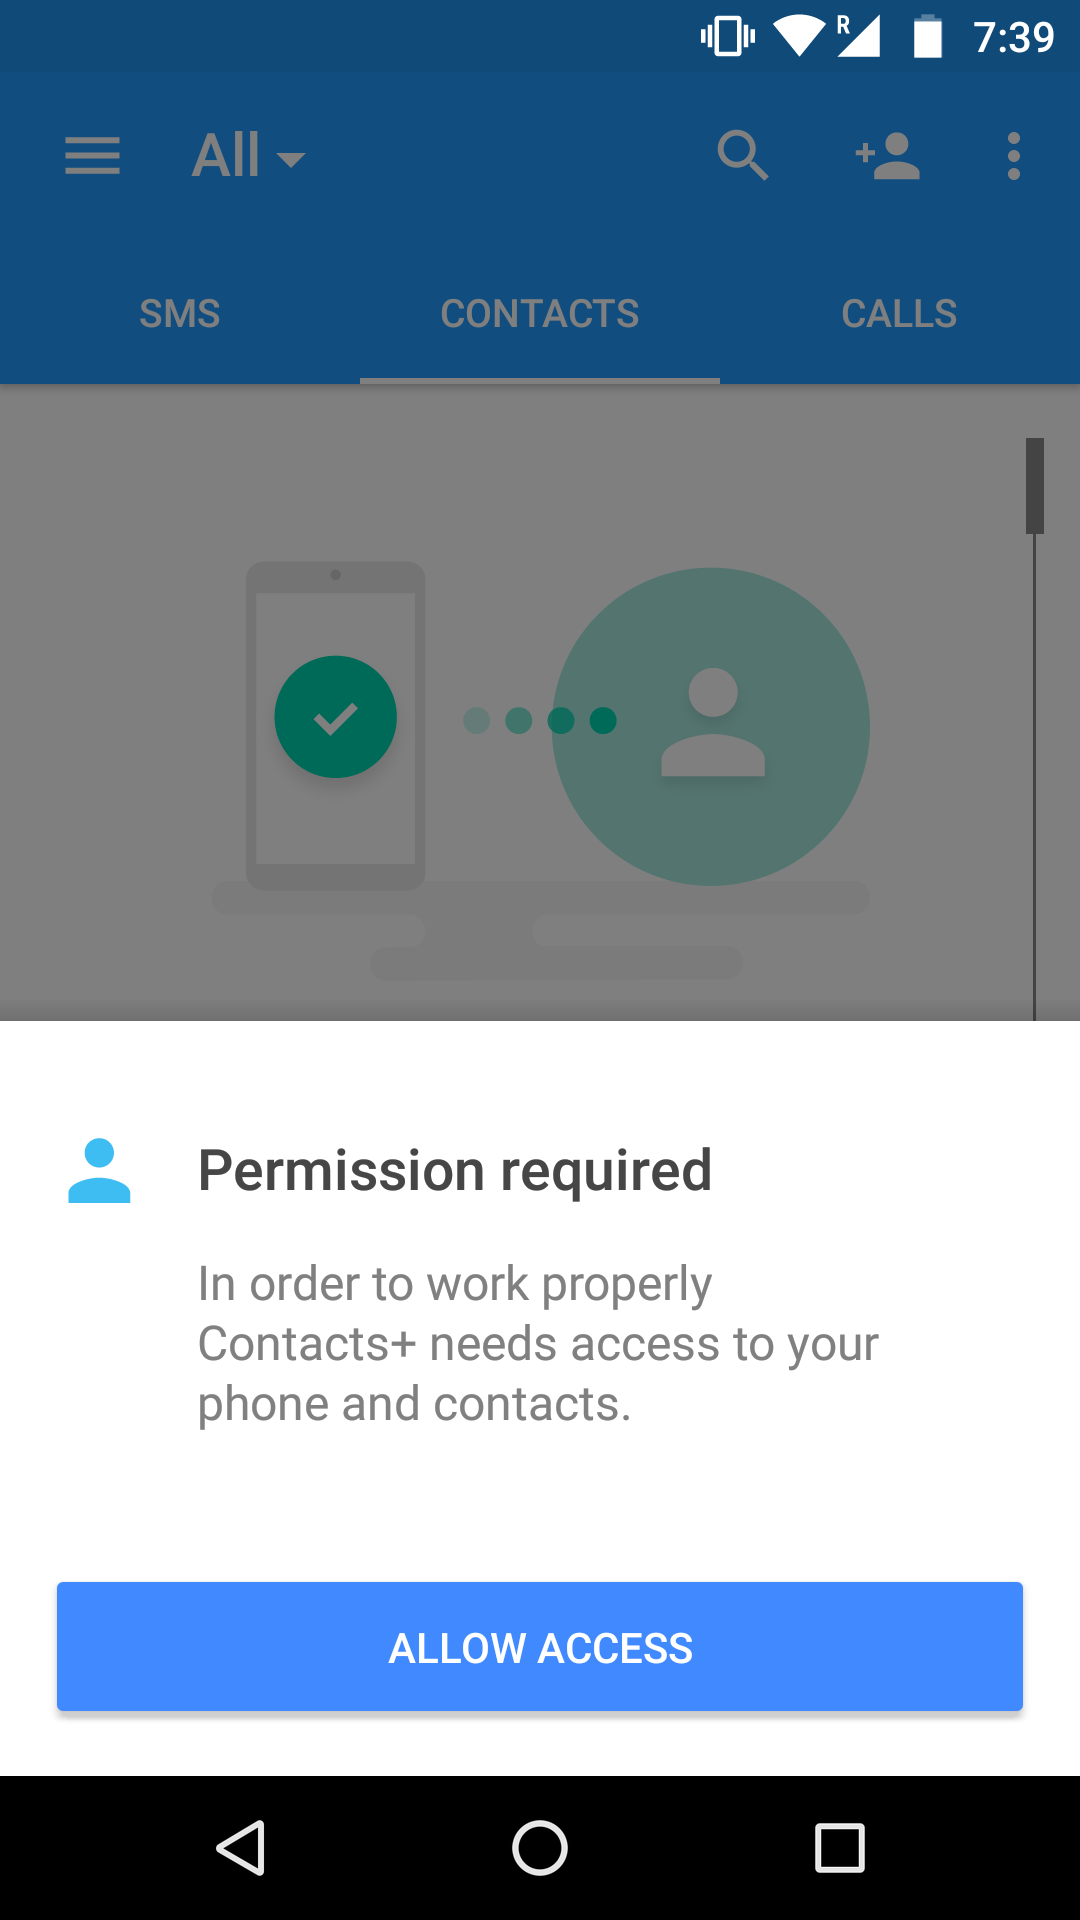
\includegraphics[width=\textwidth]{restrict_prob1.png}
		\caption{When permission to access phone is denied.}
	\end{subfigure}
	\hfill
	\begin{subfigure}[h]{0.45\textwidth}
		\centering
		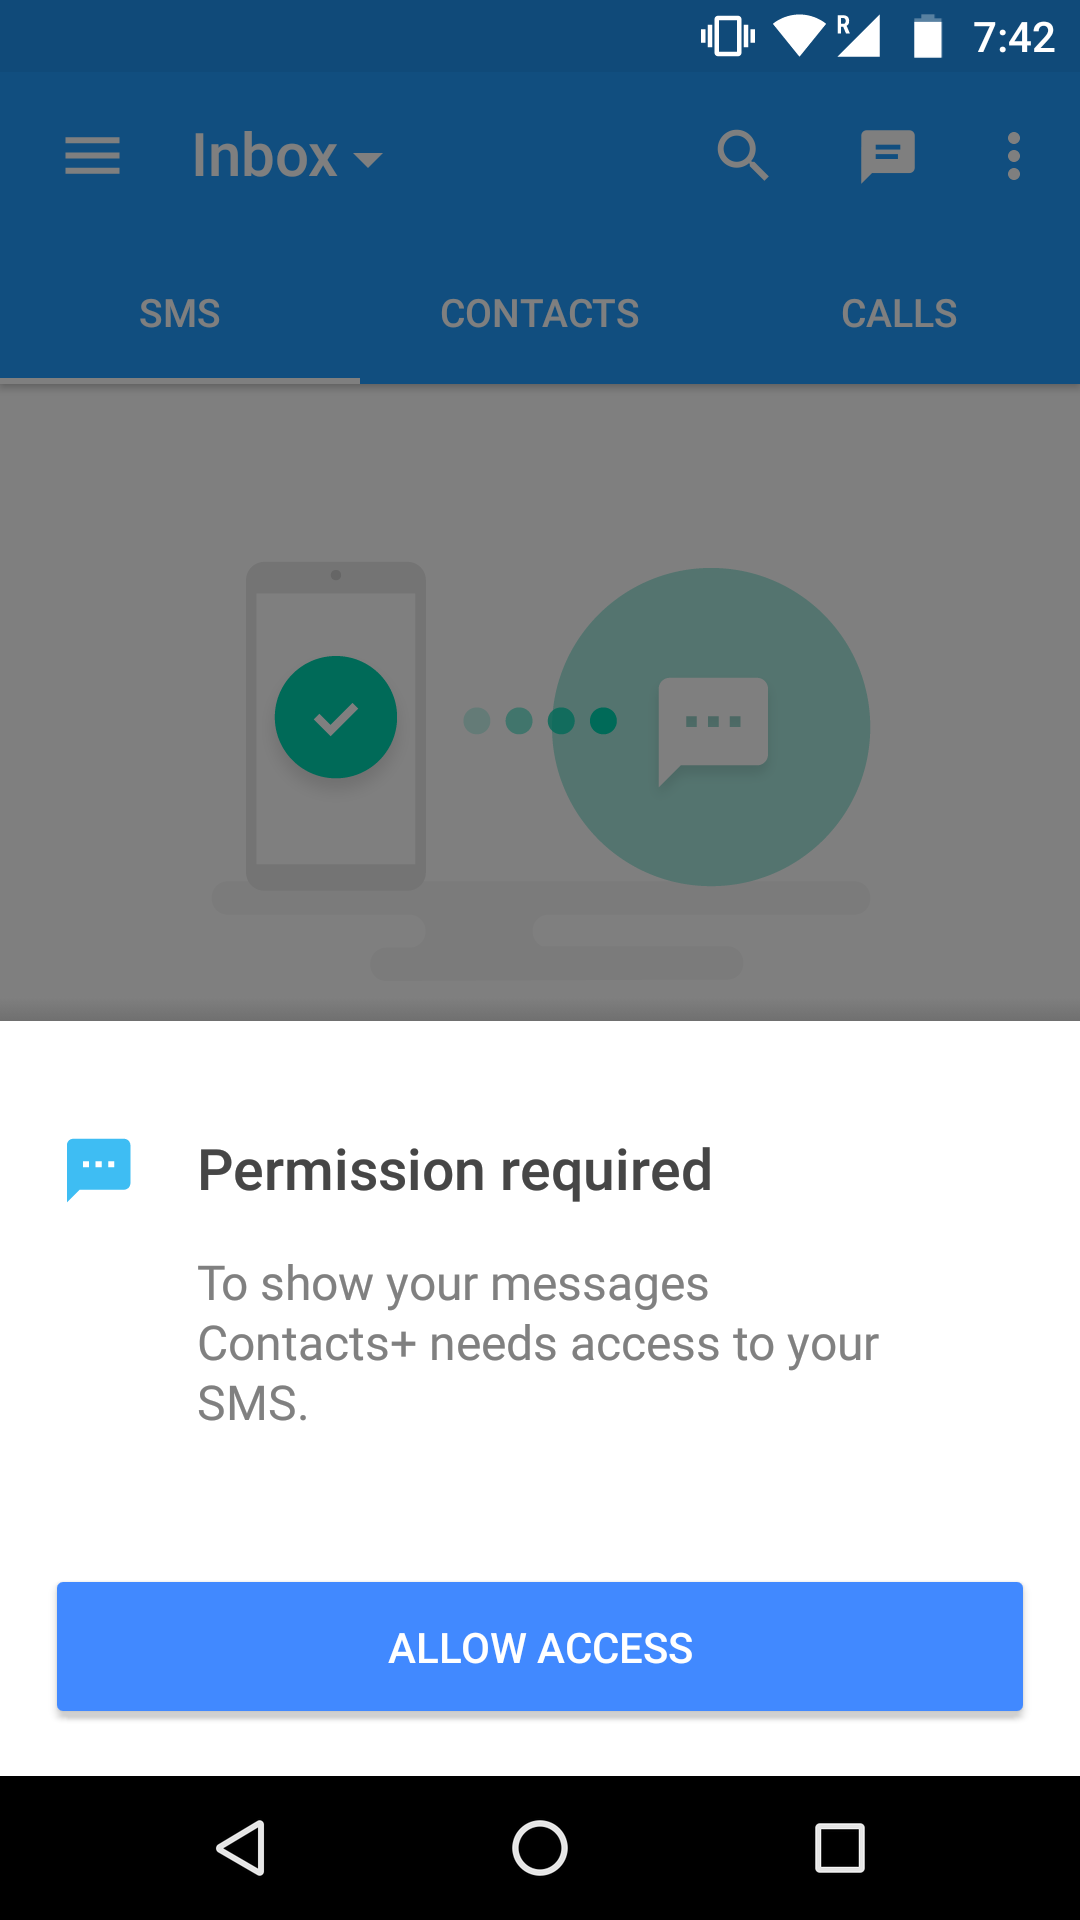
\includegraphics[width=\textwidth]{restrict_prob2.png}
		\caption{When permission to access message is denied.}
	\end{subfigure}
	\caption{Problems in Android current security scheme}
	\label{fig:prob1}
\end{figure}

Apart from the permissions, there are more things that can be used to exploit the private data of user and also can be used to degrade the performance of the device itself. Some of those are clipboard, view, etc. Clipboard is buffer which is used to hold the data copied from any application. Since clipboard is accessible to all applications, any application can read the data from clipboard and can send it to third party server. Currently, we can to stop applications from accessing clipboard data. Some applications opens the browser via link. We can stop link from opening in the browser.

Currently if an application asks permission to access message, then application will get permissions for both send message and read message. If we want to restrict an application such that it can read message but can not send. In other words, we want to control the permission of application at API level. But currently this feature is not provided by Android operating system.

We have to restrict the malicious behaviour of applications. Since, currently every application runs in its own process, with its own instance of the Dalvik virtual machine (DVK)/ Android runtime (ART). So, we can not restrict applications by developing another at fifth layer of the Android software stack. One way to restrict the malicious behaviour of applications is by modifying the Android Package (APK) file. For modifying the APK file, we have to decompile it and it convert it into smali and then we can change code of application. Smali is more of assembly based language so making change in smali is tedious task. Another way to restrict applications is without modifying the APK file. We can restrict applications at the system level by modifying the Random access memory (ROM). We have used Xposed framework \cite{xposedframework} to achieve this.\\ \\
\section{Wrapping Applicaitons}
Xposed is framework for module which can restrict or change the behaviour of the system and applications without touching any APKs. Xposed works at system level so your device should be rooted. Instead of modifying corresponding DEX or ART representation of the application, it is deeply integrated with the Android system where it replaces some system components after backing up the originals. There are multiple advantages to this approach. Some of them are:
\begin{itemize}
    \item you can modify parts of the system you otherwise could not.
    \item you can apply multiple modifications to the same app in a combination best fitting your intentions.
    \item changes are easy to undo: As all changes are done in the memory, you just need to deactivate the module and reboot to get your original system back.
\end{itemize}

Zygote is the main process of the Android runtime. Every application is started as  a copy (``fork") of it. So, this process is also called as the head of Android runtime. This process is started by an \textit{/int.rc} script when your phone is booted. The process is done with \textit{/system/bin/app\_process}, which loads the needed classes and invokes the initialization methods.

\begin{figure}[h]
	\centering
	\begin{subfigure}[h]{0.45\textwidth}
		\centering
		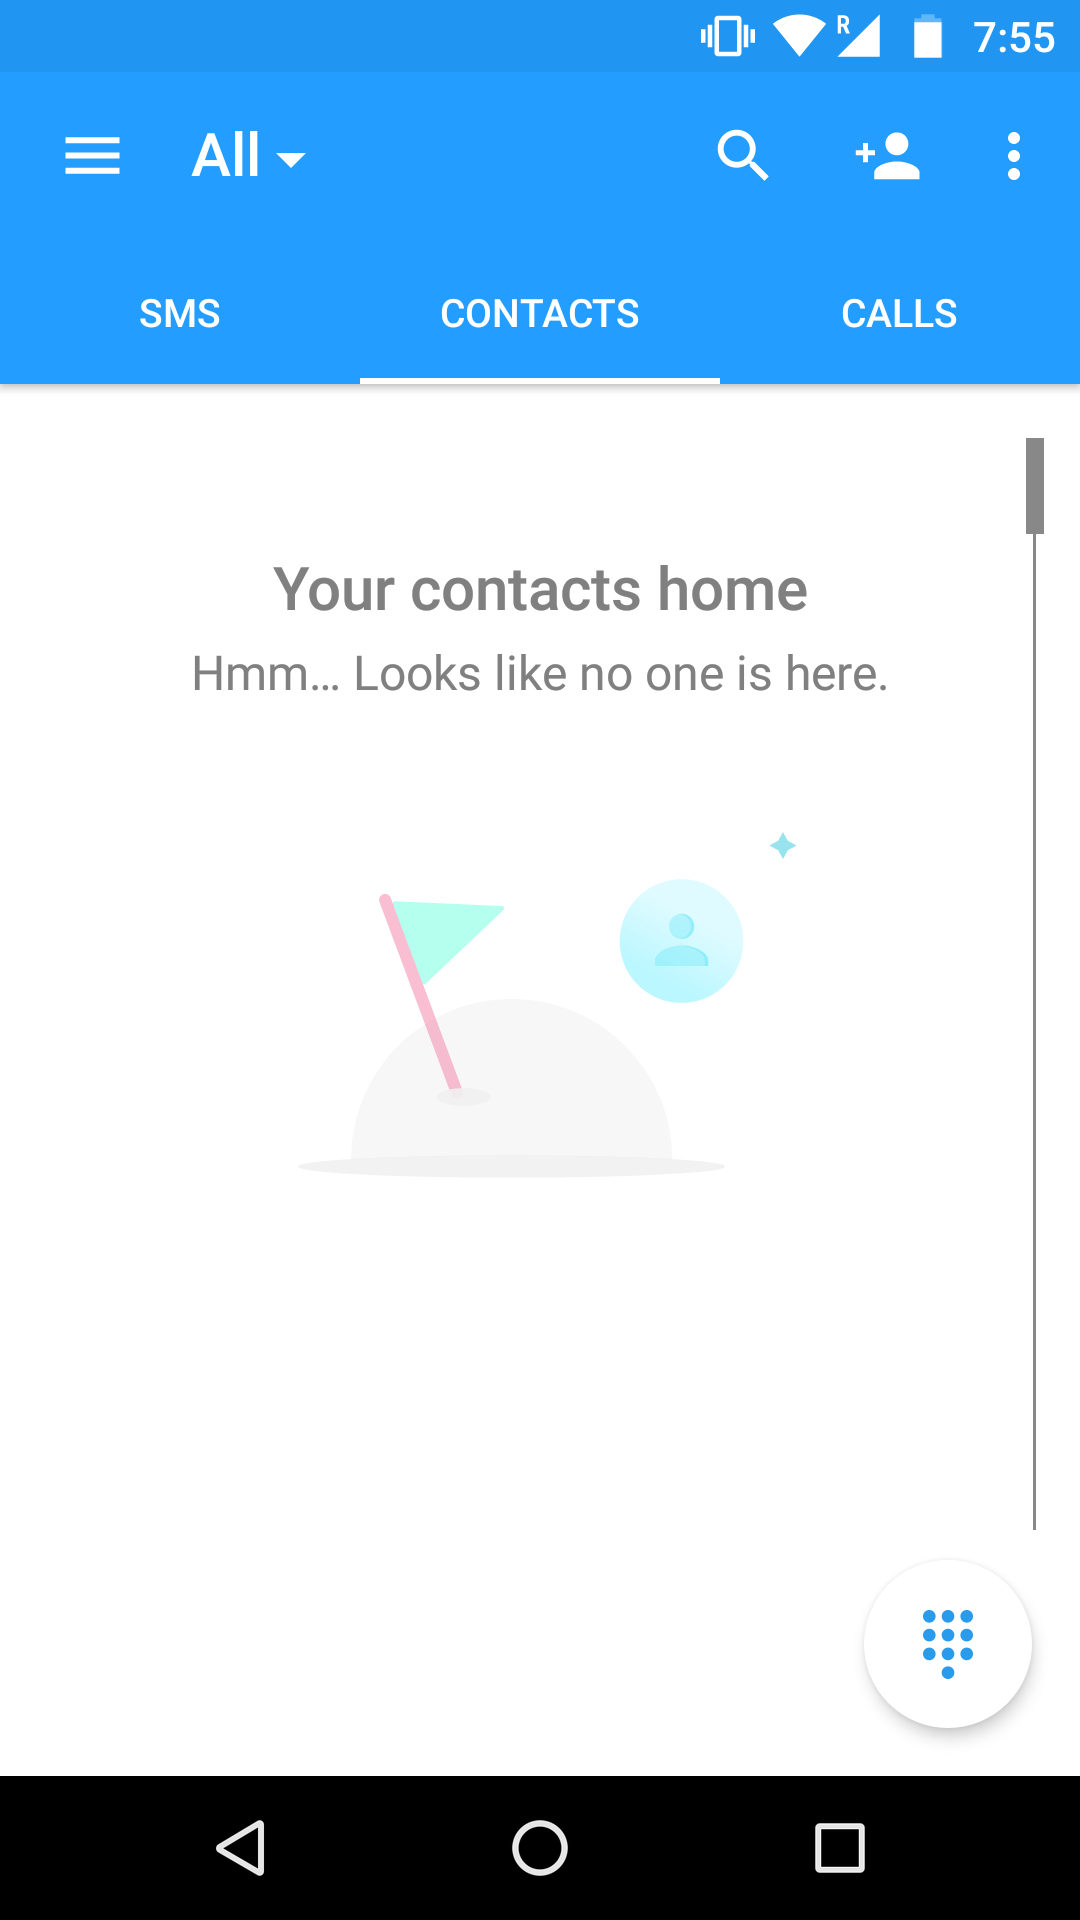
\includegraphics[width=\textwidth]{restrict_sol1.png}
		\caption{When permission to access phone is denied.}
	\end{subfigure}
	\hfill
	\begin{subfigure}[h]{0.45\textwidth}
		\centering
		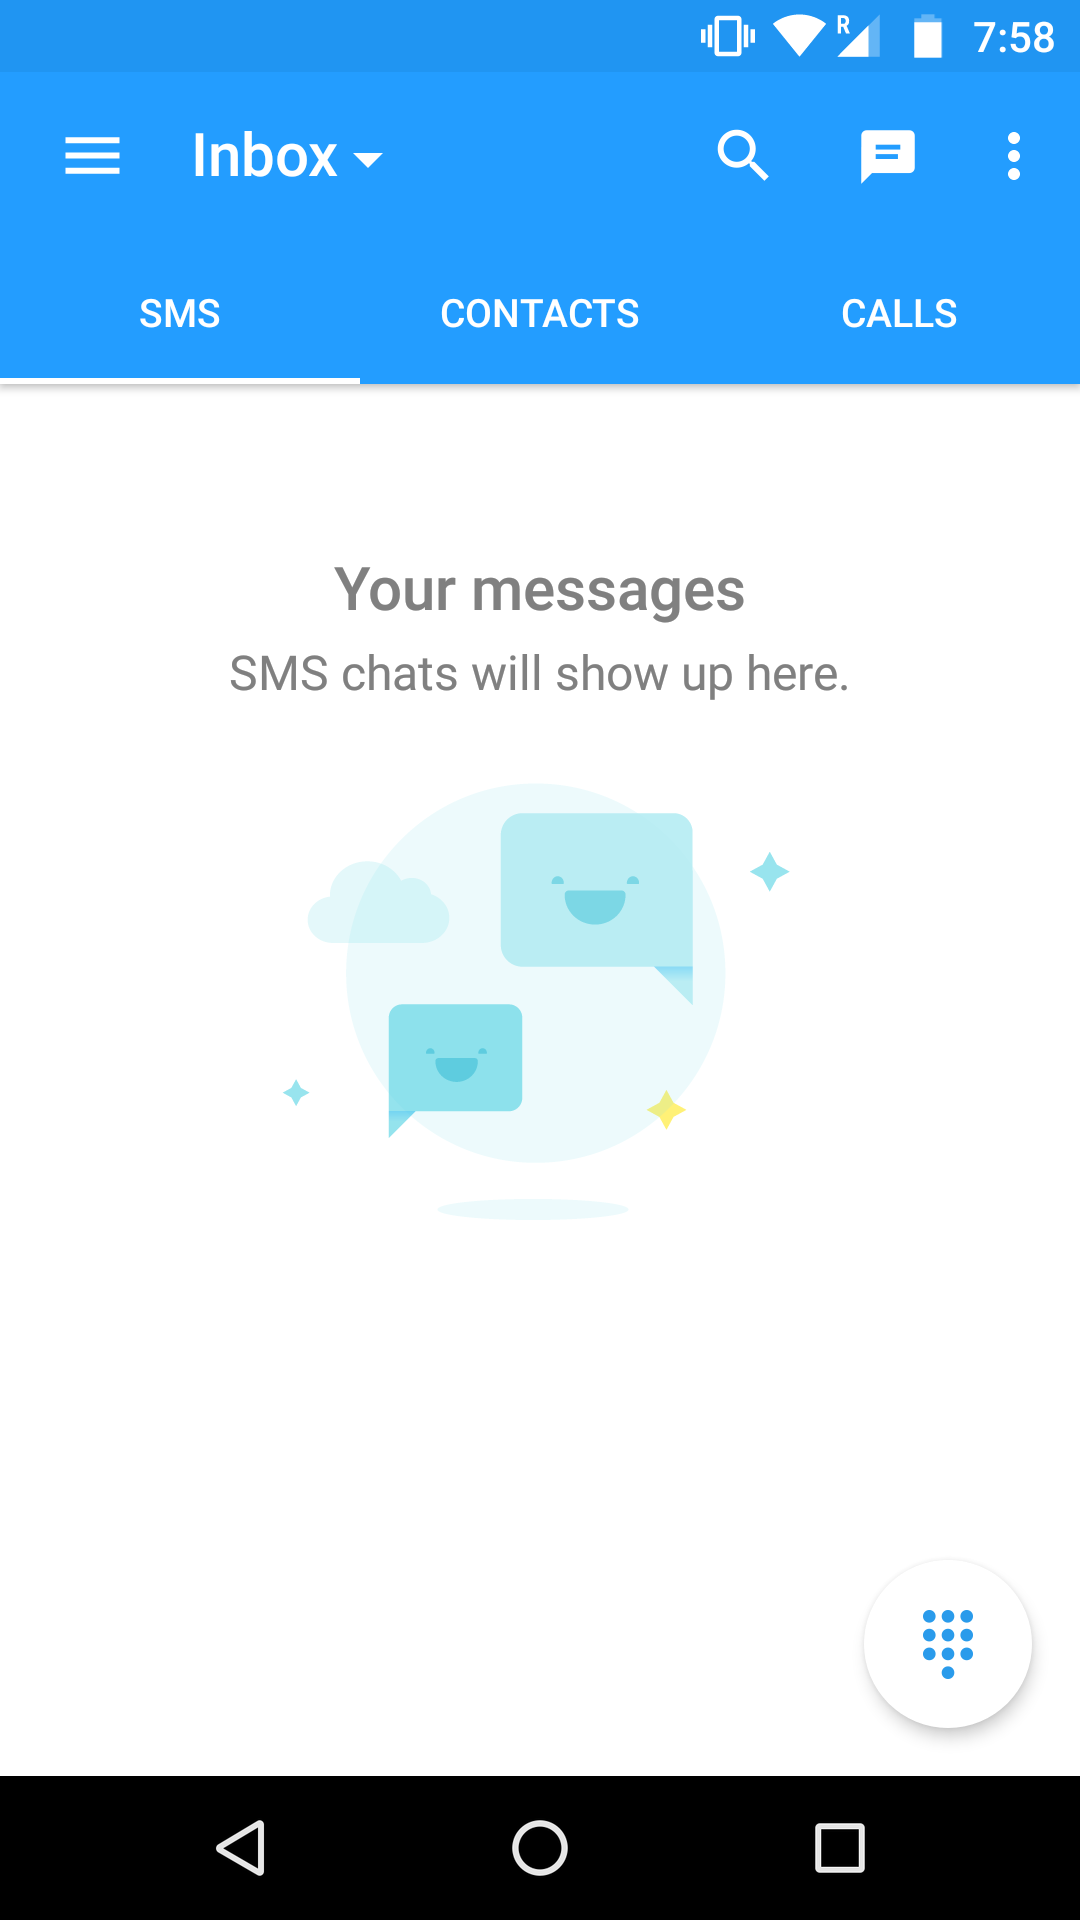
\includegraphics[width=\textwidth]{restrict_sol2.png}
		\caption{When permission to access message is denied.}
	\end{subfigure}
	\caption{App working properly after restrictions}
	\label{fig:prob2}
\end{figure}

Xposed framework creates an extended version of existing app\_process. When you install the framework, a modified and extended app\_process is copied to \textit{/sytem/bin}. This extended startup process adds an additional jar to the classpath and calls methods from there at certain places. For instance, just after the VM has been created, even before the main method of Zygote has been called. And inside that method, we are part of Zygote and can act in its context. So, now we can control
the method calls of other application from there.

To provide the security, we have to restrict the method calls from the application. When an application calls any method, we can do three things with that method. Either we can change the parameter of method or we can change body of the method. We can also leave the method unmodified. We have modified the existing modules of Xposed framework to control the methods. Now, if an application wants to access the resource, then we can feed the application with no data of fake data. We have restricted the applications from accessing contacts and messages. Since Xposed module does not revoke or block permissions from an application, so most application will continue to work as before and won't force close or crash as shown in Figure \ref{fig:prob2}. Now, we can also control the applications at API level. We can also restrict the application from pasting the data from clipboard either manually or automatically.
\section{Implementation}
Android provides different layers of software stack to handle different things. Currently, if an application invokes any methods, it is handled by Binder IPC module. Binder IPC module binds the method with native libraries. Interaction between apps, application framework, and linux kernel on Android is shown in Figure \ref{fig:impl1}.
\begin{figure}[!h]
  \centering
  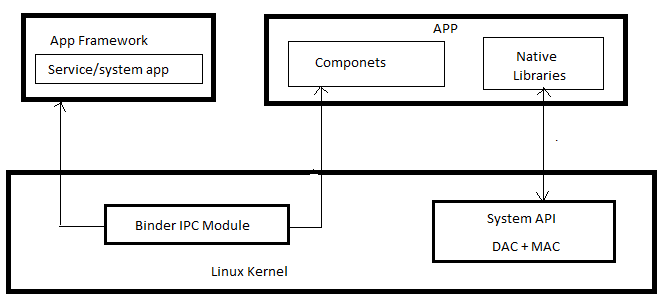
\includegraphics [scale=0.8] {impl1.png}
  \caption{Interaction between apps, application framework, and Linux kernel on Android}
  \label{fig:impl1}
\end{figure}

Xposed framework modifies the \textit{app\_process} file of \textit{/sytem/bin} and adds an extra jar file to Android to intercept the methods. Since, it modifies the \textit{app\_process} and every other process is child process of \textit{app\_process}, so Xposed becomes the integral part of the every methods. Workflow of Xposed framework is shown in Figure \ref{fig:impl2}.
\begin{figure}[!h]
  \centering
  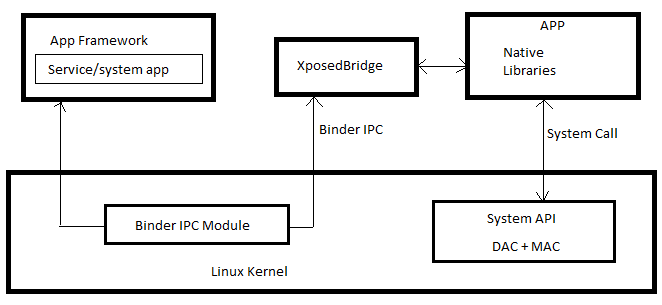
\includegraphics [scale=0.8] {impl2.png}
  \caption{Interaction between apps, application framework, and Linux kernel on Android}
  \label{fig:impl2}
\end{figure}

Xposed framework provides mechanism to intercept method calls of any application. Xposed provides \texttt{handleHookedMethod} to handle the methods call of applications. Using this method we can modify the parameters of method, or body of methods. It also provides two more methods namely \texttt{beforeHookedMethod} and \texttt{afterHookedMethod}. We can modify this method to achieve the desired results. We have modified the existing modules of exposed framework to restrict different permissions. We have modified it such that it gives the fake data or no data to the applications, so applications work properly.
\section{Case Study}
We have analyzed 10 applications. After analyzing, we have categorized the applications into classes namely benign and malicious. Following applications have been labelled as the benign:
\begin{spacing}{0.9}
\begin{itemize}
    \item Budget Planner
    \item BHIM Making India Cashless
    \item Tez: A new payment app by Google
    \item Google Calendar
\end{itemize}
\end{spacing}
Since, these applications are benign we do not have to restrict any permissions of the applications. Following applications have been labelled as the malicious:
\begin{spacing}{0.9}
\begin{itemize}
    \item Funnyys
    \item Omingo
    \item System Certificate
    \item MMS Beline
    \item Laughtter
    \item Android Framework
\end{itemize}
\end{spacing}
Since, these applications are malicious we have restricted its malicious behaviour by wrapping it. Permissions which are causing malicious behaviour is denied.\\
{\Large \textbf{Funnyys}}\\
Funnys is an online game applications, so it does not require permissions to access message, phone and camera. So we have restricted the following permissions:

\begin{itemize}
\begin{spacing}{0.9}
\item \texttt{android.permission.SEND\_SMS}
\item \texttt{android.permission.RECEIVE\_SMS}
\item \texttt{android.permission.WRITE\_SMS}
\item \texttt{android.permission.READ\_SMS}
\item \texttt{android.permission.CAMERA}
\end{spacing}
\end{itemize}
{\Large\textbf{Omingo}}\\
This app lets hackers control your device, giving them unauthorized access to your data. To prevent the malicious behaviour of this application, we have restricted following permissions:

\begin{itemize}
\begin{spacing}{0.9}
\item \texttt{android.permission.RECEIVE\_SMS}
\item \texttt{android.permission.SEND\_SMS}
\item \texttt{android.permission.WRITE\_APN\_SETTINGS}
\item \texttt{android.permission.CLEAR\_APP\_CACHE}
\item \texttt{android.permission.READ\_SMS}
\item \texttt{android.permission.RECEIVE\_WAP\_PUSH}
\item \texttt{android.permission.INSTALL\_PACKAGES}
\item \texttt{android.permission.CLEAR\_APP\_USER\_DATA}
\item \texttt{android.permission.MOUNT\_UNMOUNT\_FILESYSTEMS}
\item \texttt{android.permission.RECEIVE\_BOOT\_COMPLETED}
\item \texttt{android.permission.DELETE\_CACHE\_FILES}
\item \texttt{android.permission.WRITE\_EXTERNAL\_STORAGE}
\item \texttt{android.permission.REBOOT}
\item \texttt{android.permission.RESTART\_PACKAGES}
\item \texttt{android.permission.DELETE\_PACKAGES}
\end{spacing}
\end{itemize}
{\Large \textbf{System Certificate}}\\
System Certificate  is a fake application which can damage your device and steal your data. To stop its malicious intent, we have restricted the following permissions:
\begin{itemize}
    \item \texttt{android.permission.INTERNET}
\end{itemize}\\
{\Large \textbf{MMS Beline}}\\
MMS Beline is a third party application which can increase your mobile bill by sending message and by calling to the premium number. This application is installed by another malicious applications. It runs in background. We have to uninstall this application because this application is of no use.\\
{\Large \textbf{Lughtter}}\\
It is another application which can add charges to your mobile bill by sending costly SMS message without informing you first. So we have restricted the following permissions:

\begin{itemize}
\begin{spacing}{0.9}
    \item \texttt{android.permission.SEND\_SMS}
\item \texttt{android.permission.RECEIVE\_SMS}
\item \texttt{android.permission.WRITE\_SMS}
\item \texttt{android.permission.READ\_SMS}
\item \texttt{android.permission.CAMERA}
\item \texttt{android.permission.READ\_PHONE\_STATE}
\end{spacing}
\end{itemize}
{\Large\textbf{Android Framework}}\\
Android Framework is a third party application which can increase your mobile bill by sending message and by calling to the premium number. It can install other malicious applications to your device. So we have to uninstall this application. \\
{\Large \textbf{Duet}}\\
Duet is a game. We have restricted access to identification, internet, location, phone, and view. Though, we have restricted some access for application still it is working properly. Figure \ref{fig:duet} shows the screenshot of application working properly after restrictions.

\begin{figure}[h]
	\centering
	\begin{subfigure}[h]{0.45\textwidth}
		\centering
		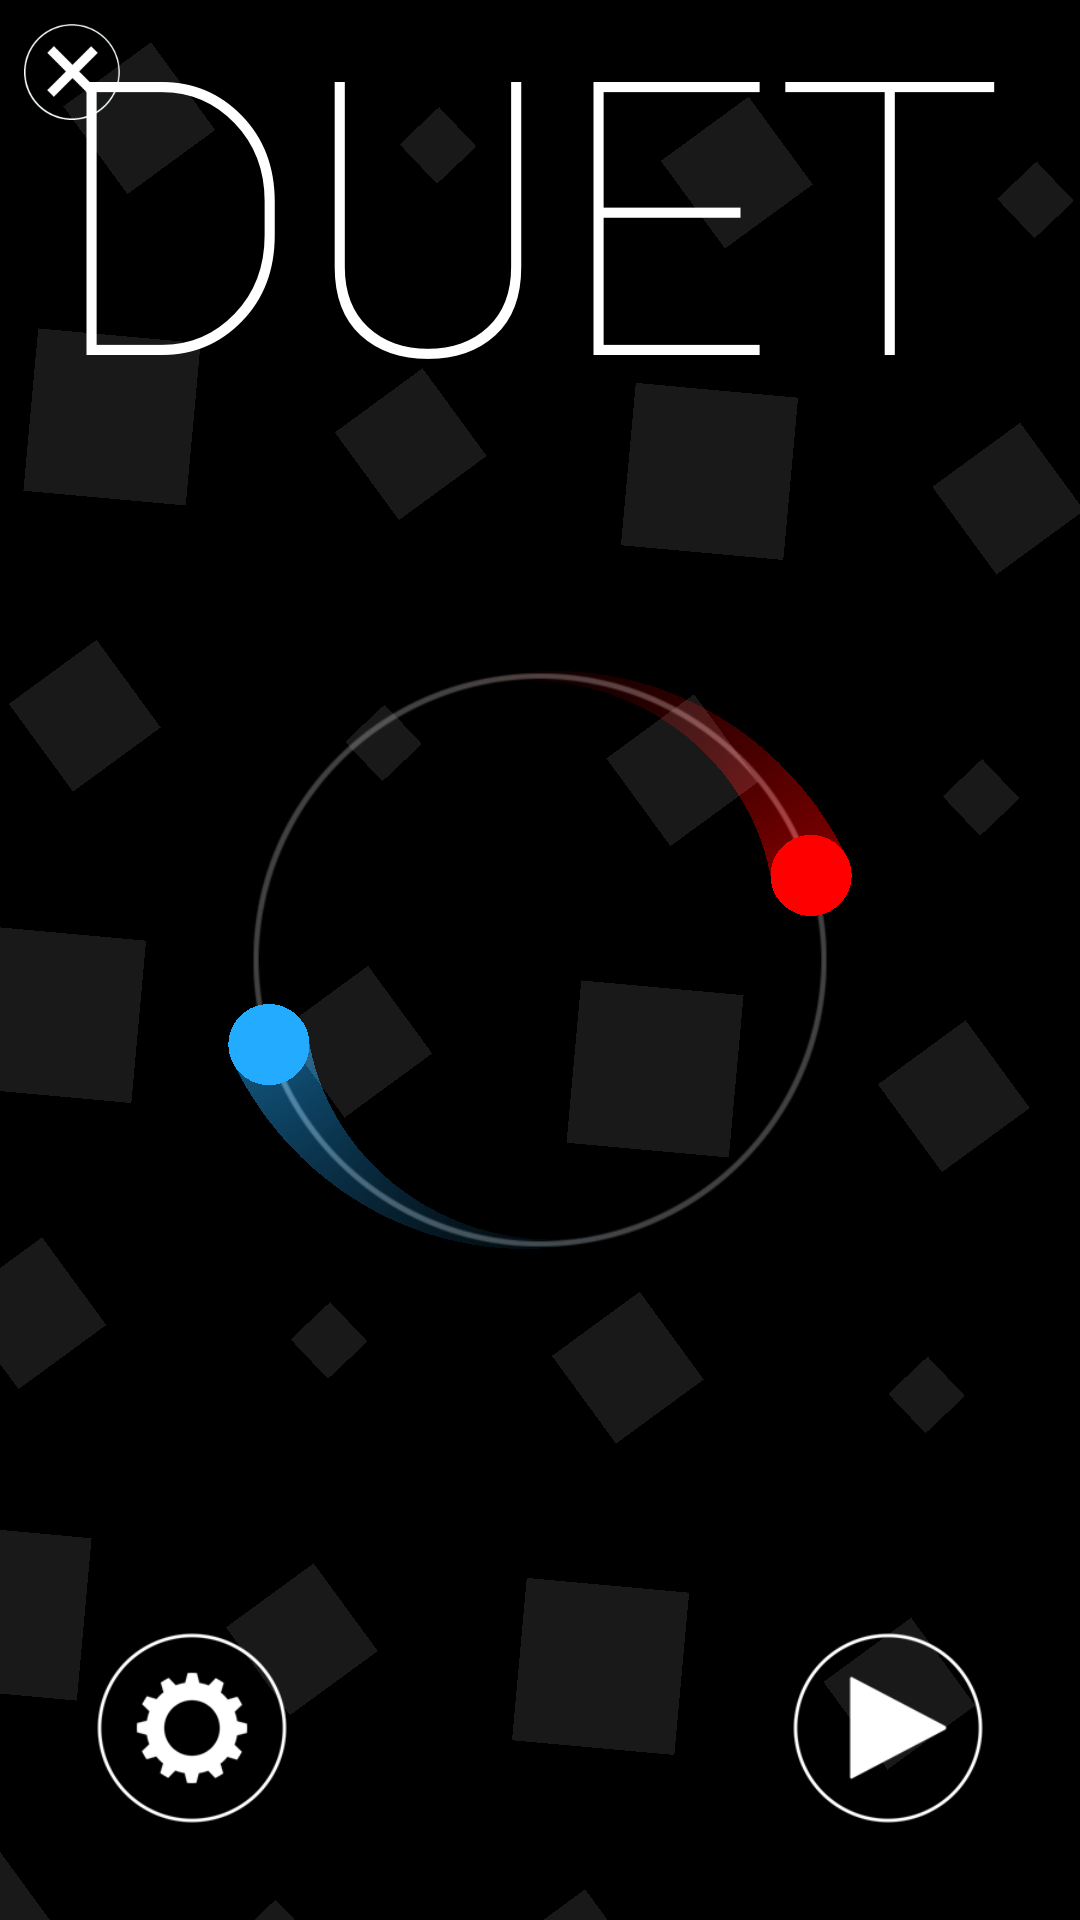
\includegraphics[width=\textwidth]{duet1.png}
		\caption{Screenshot- 1}
	\end{subfigure}
	\hfill
	\begin{subfigure}[h]{0.45\textwidth}
		\centering
		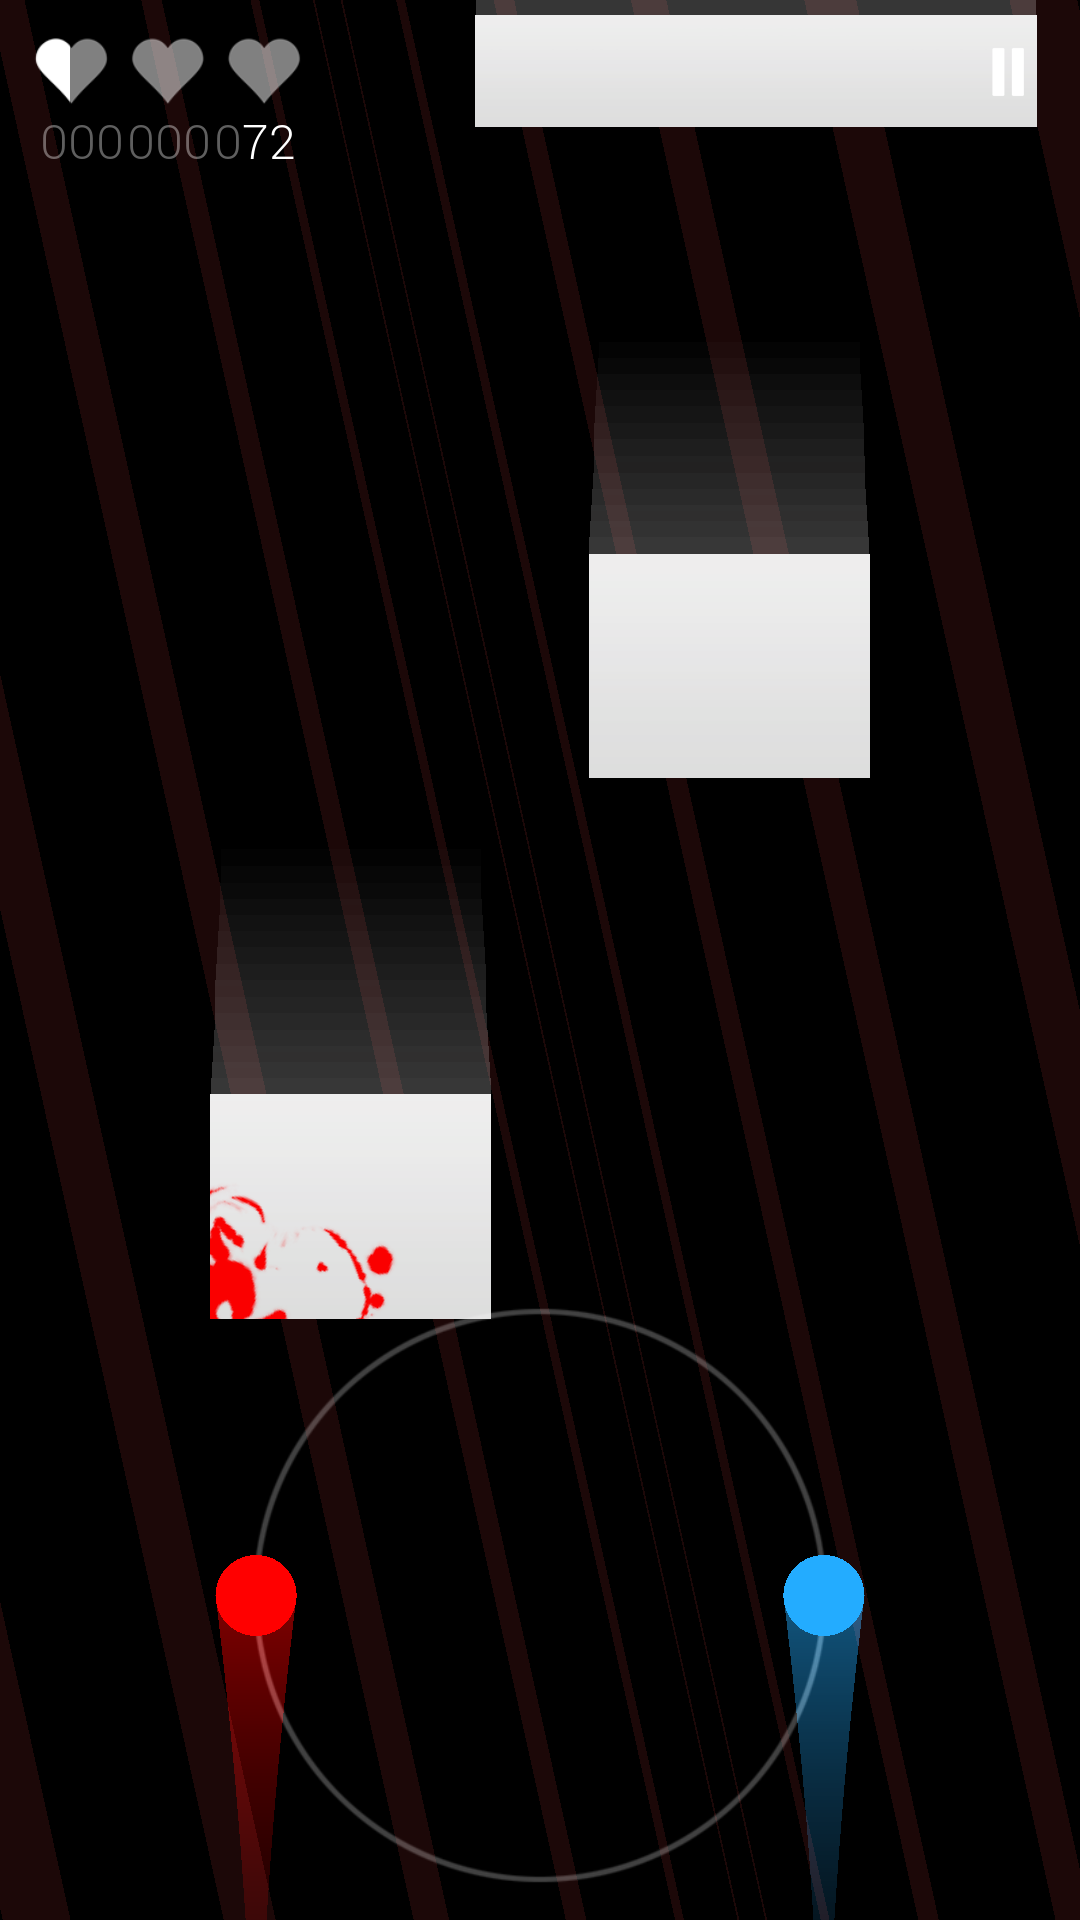
\includegraphics[width=\textwidth]{duet2.png}
		\caption{Screenshot- 2}
	\end{subfigure}
	\caption{App working properly after restrictions}
	\label{fig:duet}
\end{figure}
%% Main chapter title
\chapter{Case Study}
\label{ch:dl}

% This is for the header on each page
\lhead{Chapter 4. \emph{Case Study}}

We have analyzed 10 applications. After analyzing, we have categorized the applications into classes namely benign and malicious. Following applications have been labelled as the benign:
\begin{itemize}
    \item Budget Planner
    \item BHIM Making India Cashless
    \item Tez: A new payment app by Google
    \item Google Calendar
\end{itemize}
Since, these applications are benign we do not have to restrict any permissions of the applications. Following applications have been labelled as the malicious:
\begin{itemize}
    \item Funnyys
    \item Omingo
    \item System Certificate
    \item MMS Beline
    \item Laughtter
    \item Android Framework
\end{itemize}

Since, these applications are malicious we have restricted its malicious behaviour by wrapping it. Permissions which are causing malicious behaviour is denied.\\
{\Large \textbf{Funnyys}}\\
Funnys is an online game applications, so it does not require permissions to access message, phone and camera. So we have restricted the following permissions for Funnys application:
\begin{itemize}
    \item \texttt{android.permission.SEND\_SMS}
\item \texttt{android.permission.RECEIVE\_SMS}
\item \texttt{android.permission.WRITE\_SMS}
\item \texttt{android.permission.READ\_SMS}
\item \texttt{android.permission.CAMERA}
\item \texttt{android.permission.READ\_PHONE\_STATE}
\end{itemize}\\
{\Large \textbf{Omingo}}\\
This app lets hackers control your device, giving them unauthorized access to your data. To prevent the malicious behaviour of this application, we have restricted following permissions:
\begin{itemize}
    \item \texttt{android.permission.RECEIVE\_SMS}
\item \texttt{android.permission.SEND\_SMS}
\item \texttt{android.permission.WRITE\_APN\_SETTINGS}
\item \texttt{android.permission.CLEAR\_APP\_CACHE}
\item \texttt{android.permission.READ\_SMS}
\item \texttt{android.permission.RECEIVE\_WAP\_PUSH}
\item \texttt{android.permission.INSTALL\_PACKAGES}
\item \texttt{android.permission.CLEAR\_APP\_USER\_DATA}
\item \texttt{android.permission.MOUNT\_UNMOUNT\_FILESYSTEMS}
\item \texttt{android.permission.RECEIVE\_BOOT\_COMPLETED}
\item \texttt{android.permission.DELETE\_CACHE\_FILES}
\item \texttt{android.permission.WRITE\_EXTERNAL\_STORAGE}
\item \texttt{android.permission.REBOOT}
\item \texttt{android.permission.RESTART\_PACKAGES}
\item \texttt{android.permission.DELETE\_PACKAGES}
\end{itemize}\\
{\Large \textbf{System Certificate}}\\
System Certificate  is a fake application which can damage your device and steal your data. To stop its malicious intent, we have restricted the following permissions:
\begin{itemize}
    \item \texttt{android.permission.INTERNET}
\end{itemize}\\
{\Large \textbf{MMS Beline}}\\
MMS Beline is a third party application which can increase your mobile bill by sending message and by calling to the premium number. This application is installed by another malicious applications. It runs in background. We have to uninstall this application because this application is of no use.\\
{\Large \textbf{Lughtter}}\\
It is another application which can add charges to your mobile bill by sending costly SMS message without informing you first. So we have restricted the following permissions:
\begin{itemize}
    \item \texttt{android.permission.SEND\_SMS}
\item \texttt{android.permission.RECEIVE\_SMS}
\item \texttt{android.permission.WRITE\_SMS}
\item \texttt{android.permission.READ\_SMS}
\item \texttt{android.permission.CAMERA}
\item \texttt{android.permission.READ\_PHONE\_STATE}
\end{itemize}\\
{\Large \textbf{Android Framework}}\\
Android Framework is a third party application which can increase your mobile bill by sending message and by calling to the premium number. It can install other malicious applications to your device. So we have to uninstall this application.
{\Large \textbf{Duet}}\\
Duet is a game. We have restricted access to identification, internet, location, phone, and view. Though, we have restricted some access for application still it is working properly. 
% Main chapter title
\chapter{Conclusion and Future Work}
\label{ch:dl}

% This is for the header on each page
\lhead{Chapter 4. \emph{Conclusion and Future Work}}
\thispagestyle{empty}
In this work we have presented 4 different machine learning models that are trained on a well-known permission classification dataset. We could improve the identification and classification on Android apps with higher accuracy than the available current methods. We have presented our approach with running case studies on a few Android apps and presented our tool's accuracy in identification of malicious apps. Our approach involved a mix of static and dynamic analysis such that even the apps that have unused APIs present in the code that can be traversed post classification of the app as benign by the application store. We have restricted the malicious behaviour of application without interrupting its execution.


%Our tool restricts applications from performing any malicious activity. For restricting the malicious behaviour of application, we have analyzed the application using both dynamic and static analysis. After doing analysis, we have proposed the possible description of applications. After analysis, we have classified the applications as benign or malicious. After identifying the malicious application, we have restricted the malicious behaviour of application.\\

As an extension of this work, one may automate the process of permission classification of installed apps.
Currently, we are manually deciding which permissions are causing malicious behaviour in a particular application. We can integrate our app classification model with a tool which can give the list permissions which are causing the malicious behaviour.


\appendix % Cue to tell LaTeX that the following 'chapters' are Appendices

% Import the Appendices
% \input{AppendixA}

\backmatter

% This file contains the templates for the last few pages of the thesis including 
% 1. List of publications
% 2. Acknowledgements

% \newcommand{\publications}{

% Page number at bottom
% \thispagestyle{plain}

% Title
% \begin{center}{\huge{\textbf{List of Publications}} \par}\end{center}

% \vspace*{15px}

% List your publications here

% 1.

% 2.
% }

\newcommand{\acknowledgements}{

% Page number at bottom
\thispagestyle{plain}

% Title
\begin{center}{\huge{\textit{Acknowledgements}} \par}\end{center}

\vspace*{15px}

% Write acknowledgement here

I am thankful to my supervisor \textbf{Prof. R.K. Shyamasundar} for his enormous support and insightful suggestions throughout my project. I am grateful to him for providing me his code base support which was very useful in carrying out my experiments. His insightful suggestions to the various problems that I faced during my project, were not only useful, but also helped me in broadening my basic understanding of project area. I am also thankful to \textbf{Dr. Vishwas Patil} for his enormous support and suggestion throughout my project. 

\vspace*{15px}

\begin{flushright}
{Signature: ......................................\\[0.4cm]}

{\textbf{\authorName}\\[0.0cm]\rollNo\\[2.0cm]}
\end{flushright}

\begin{flushleft}
{Date:} ...... \currentmonth { } \currentyear\\
\end{flushleft}
}

% Bibliography

\label{Bibliography}
\lhead{\emph{Bibliography}}


\bibliographystyle{acl2016.bst} % Use the "unsrtnat" BibTeX style for formatting the Bibliography

\bibliography{Bibliography} % The references (bibliography) information are stored in the file named "Bibliography.bib"

\clearpage

% List of Publications
% \addcontentsline{toc}{chapter}{List of Publications}
% \publications

\clearpage

% Acknowledgements
\addcontentsline{toc}{chapter}{Acknowledgements}

\includepdf[pages=3,trim=0mm 0mm 35mm -20mm]{d_mtp}

\end{document}
% End of the document